%!TEX root = main.tex
%\ProvidesPackage{config}

%\RequirePackage{silence}
%\WarningFilter{biblatex}{Patching footnotes failed}
\documentclass[11pt]{beamer}
\usepackage[utf8]{inputenc}
\usepackage[T1]{fontenc}

\usepackage[frenchb]{babel}
\usepackage{todonotes}
\usepackage{color}
\usepackage{bm} % \bm{} for bold font in text and math modes
\usepackage{caption,subcaption} % subcaption -> \begin{subfigure}
\usepackage{relsize}
\usepackage{booktabs,tabularx}
\usepackage{pifont} % for using \ding{}


\definecolor{green2}{RGB}{0.0,0.5,0.0}
\newcommand{\cmark}{\textcolor[rgb]{0.0,0.5,0.0}{\ding{51}}}% "check" mark
\newcommand{\xmark}{\textcolor{red}{\ding{55}}}% "cross" mark
\usepackage{amsmath}
\usepackage{amssymb}
\usepackage{booktabs,tabularx}
\usepackage{tikz}
\usetikzlibrary{arrows.meta,shapes.arrows}

\usepackage[backend=biber,style=ieee-alphabetic,date=long,maxbibnames=5,language=english]{biblatex}
\renewcommand{\UrlFont}{\ttfamily}


\usetheme{Warsaw}
\usefonttheme[onlymath]{serif}
\setbeamertemplate{footline}{~\insertframenumber/\inserttotalframenumber~} % Display slide numbering "2/30"
\setbeamertemplate{navigation symbols}{}



\bibliography{master-thesis.bib}


\AtBeginSection
{
\begin{frame}
		\tableofcontents[currentsection, hideothersubsections]
\end{frame}
}

% To suppress the page numbering of References at the end
\newcommand{\backupbegin}{
   \newcounter{framenumberappendix}
   \setcounter{framenumberappendix}{\value{framenumber}}
}
\newcommand{\backupend}{
   \addtocounter{framenumberappendix}{-\value{framenumber}}
   \addtocounter{framenumber}{\value{framenumberappendix}} 
}

% Because \begin{center} adds huge whitespaces
\newenvironment{tightcenter}{%
  \setlength\topsep{0pt}
  \setlength\parskip{0pt}
  \begin{center}
}{%
  \end{center}
}
  % Les usepackage sont dans config.tex
%%%%%%%%%%%%%%%%%%%%%%%%%%%%%%%%%%%%%%%%%%%%%%%%%%%%%%%%%%%
% MACROS
%%%%%%%%%%%%%%%%%%%%%%%%%%%%%%%%%%%%%%%%%%%%%%%%%%%%%%%%%%%

% Couleurs pour les corrections
\newcommand {\JY}[1] {\textcolor{red}{#1}}
\newcommand {\FR}[1] {\textcolor[rgb]{0.0,0.3,0.0}{#1}}
\newcommand {\OL}[1] {\textcolor{blue}{#1}}
\newcommand {\HW}[1] {\textcolor[rgb]{0.3,0.2,0.0}{#1}}
%\newcommand{\hilite}[1] {\emph{#1}}
\newcommand{\hilite}[1] {\Req{#1}}
\newcommand {\Req}[1] {\textcolor[rgb]{0.75,0.0,0.0}{#1}}
\newcommand {\Geq}[1] {\textcolor[rgb]{0.0,0.5,0.0}{#1}}
\newcommand {\Beq}[1] {\textcolor[rgb]{0.0,0.15,0.60}{#1}}
\newcommand {\black}[1] {\textcolor{black}{#1}}

% Espaces mathématiques
\newcommand {\DPUN} {{\mathcal D}}
\newcommand {\DTREE} {{\mathcal D}^e}
\newcommand {\CC} {\mathbb C}
\newcommand {\RR} {\mathbb R}
\newcommand {\RP} {\mathbb R^{\mathcal P}}
\newcommand {\RPE} {\mathbb R^{\mathcal P \times |\edges |}}
\newcommand {\codeset} {\mathbb R^{\mathcal P \times \leaves}}
\newcommand {\Dset} {\mathbb R^{\mathcal P \times (\mathcal P \#\leaves) }}
\newcommand {\ZZ} {\mathbb Z}
\newcommand {\NN} {\mathbb N}
\newcommand {\PP} {{\mathcal P}}
\newcommand {\HH} {{\mathbb H}}
\newcommand {\II} {{\mathbb I}}
\renewcommand {\SS} {{\mathcal S}} % applis supports
\newcommand {\SA} {{\mathbb S}} % support accessible

% Fonctions
\newcommand {\f}[1] { {\mathcal F}\left( #1 \right) }
\newcommand {\F}[1] { {\mathcal F^{-1}}\left( #1 \right) }
\newcommand {\norm}[2] {\left\| #1 \right\| _{#2}}
\newcommand {\defeq} {\triangleq}

% Opérateurs
\DeclareMathOperator {\sign} {sign}
\DeclareMathOperator {\prox} {prox}
\DeclareMathOperator {\argmin} {argmin}
\DeclareMathOperator {\supp} {supp}
\DeclareMathOperator {\rg} {rg}
\DeclareMathOperator {\diag} {diag}
\newcommand {\RG}[1] {\rg\left( #1 \right)}
\newcommand {\SUPP}[1] {\supp\left( #1 \right)}
\newcommand {\PS}[2] {\langle #1 , #2 \rangle}
\newcommand {\PROBA}[1] {\mathbb P \left( #1 \right)}
\newcommand {\one}[1] {\mathbbm{1}_{ #1 }}
%\newcommand {\one}[1] {\chi_{ #1 }} %{\mathbbm{1}_{ #1 }}
\newcommand {\oneinf}[1] {\chi_{ #1 }}
%\newcommand {\oneinf}[1] {{\mathcal I}_{ #1 }} 

% Acronymes
\newcommand {\PSNR} { \textrm{PSNR}^* } 
\newcommand {\NRE} { \textrm{NRE} }
\newcommand {\CPR} { \textrm{RER} }
\newcommand {\COST} { \textrm{G} } % ancien compression ratio

% Raccourcis
\newtheorem{prop}{Proposition}[section]

\newcommand {\nodes} {\mathcal N}
\newcommand {\edges} {\mathcal E}
\newcommand {\leaves} {\mathcal F}
\newcommand {\NL} {\#\leaves}
\newcommand {\hall} {h^e _{e \in \edges}}
%\newcommand {\multiconv}[1] { \bigstar_{\substack{#1}}\, }
\newcommand {\multiconv}[1] { \mathbf h^{#1}\, }
\newcommand {\tpath}[1] {\mathcal{C}(#1)}
\newcommand {\code} {\mathbf x}
\newcommand {\data} {\mathbf y}
\newcommand {\dataex} {\mathbf b}
\newcommand {\databis} {\mathbf y^e}
\newcommand {\D} {\mathbf D}
\newcommand {\Hs} {\mathbf A}
\newcommand {\Ha} {\mathbf H}
\newcommand {\Haf} {\hat{\mathbf H}}
\newcommand {\Hab} {\bar{\mathbf H}}
\newcommand {\res} {\mathbf r}

\newcommand {\tree}{\mathcal T}
\newcommand{\subtree}[1]{\tree^{#1}}

\newcommand {\stopalgo}{\epsilon}

% autres MACROS
\newcommand {\hkall} {(h^k)_{1 \leq k \leq K}}
\newcommand {\hkconv} {h^1 * \dots * h^K}
\newcommand {\hkconvnorm} {\frac{h^1}{\norm{h^1}{2}} * \dots * \frac{h^K}{\norm{h^K}{2}}}
\newcommand {\hkconvp} {g^{1} * \dots * g{K}}
\newcommand {\hkconvs} {f^{1} * \dots * f^{K}}
\newcommand {\fobj} {\| \code * h^1 * \dots * h^K - \data \|_2^2}
\newcommand {\fobjlambda} {\| \lambda \code * h^1 * \dots * h^K - \data \|_2^2} % 



\title{Optimisation de dictionnaires structurés en arbres de convolutions}
\subtitle{pour la représentation parcimonieuse d'images}


\author{Maël Valais}
\institute{Collaboration IMT et IRIT-ENSEEIHT\\
	\vspace{0.2cm}
	Encadré par\\
	François Malgouyres (IMT)\\
	Jean-Yves Tourneret (IRIT-ENSEEIHT)\\
	Herwig Wendt (CNRS-ENSEEIHT)
}
\date{Soutenance de stage du 8 septembre 2016}



\begin{document}

\maketitle

\section{Introduction}
\subsection{La représentation parcimonieuse}

\begin{frame}{La représentation parcimonieuse}
Représenter parcimonieusement = trouver une représentation d'une image avec un maximum de \alert{coefficients à zéro}
\begin{figure}\centering
\makebox[\linewidth]{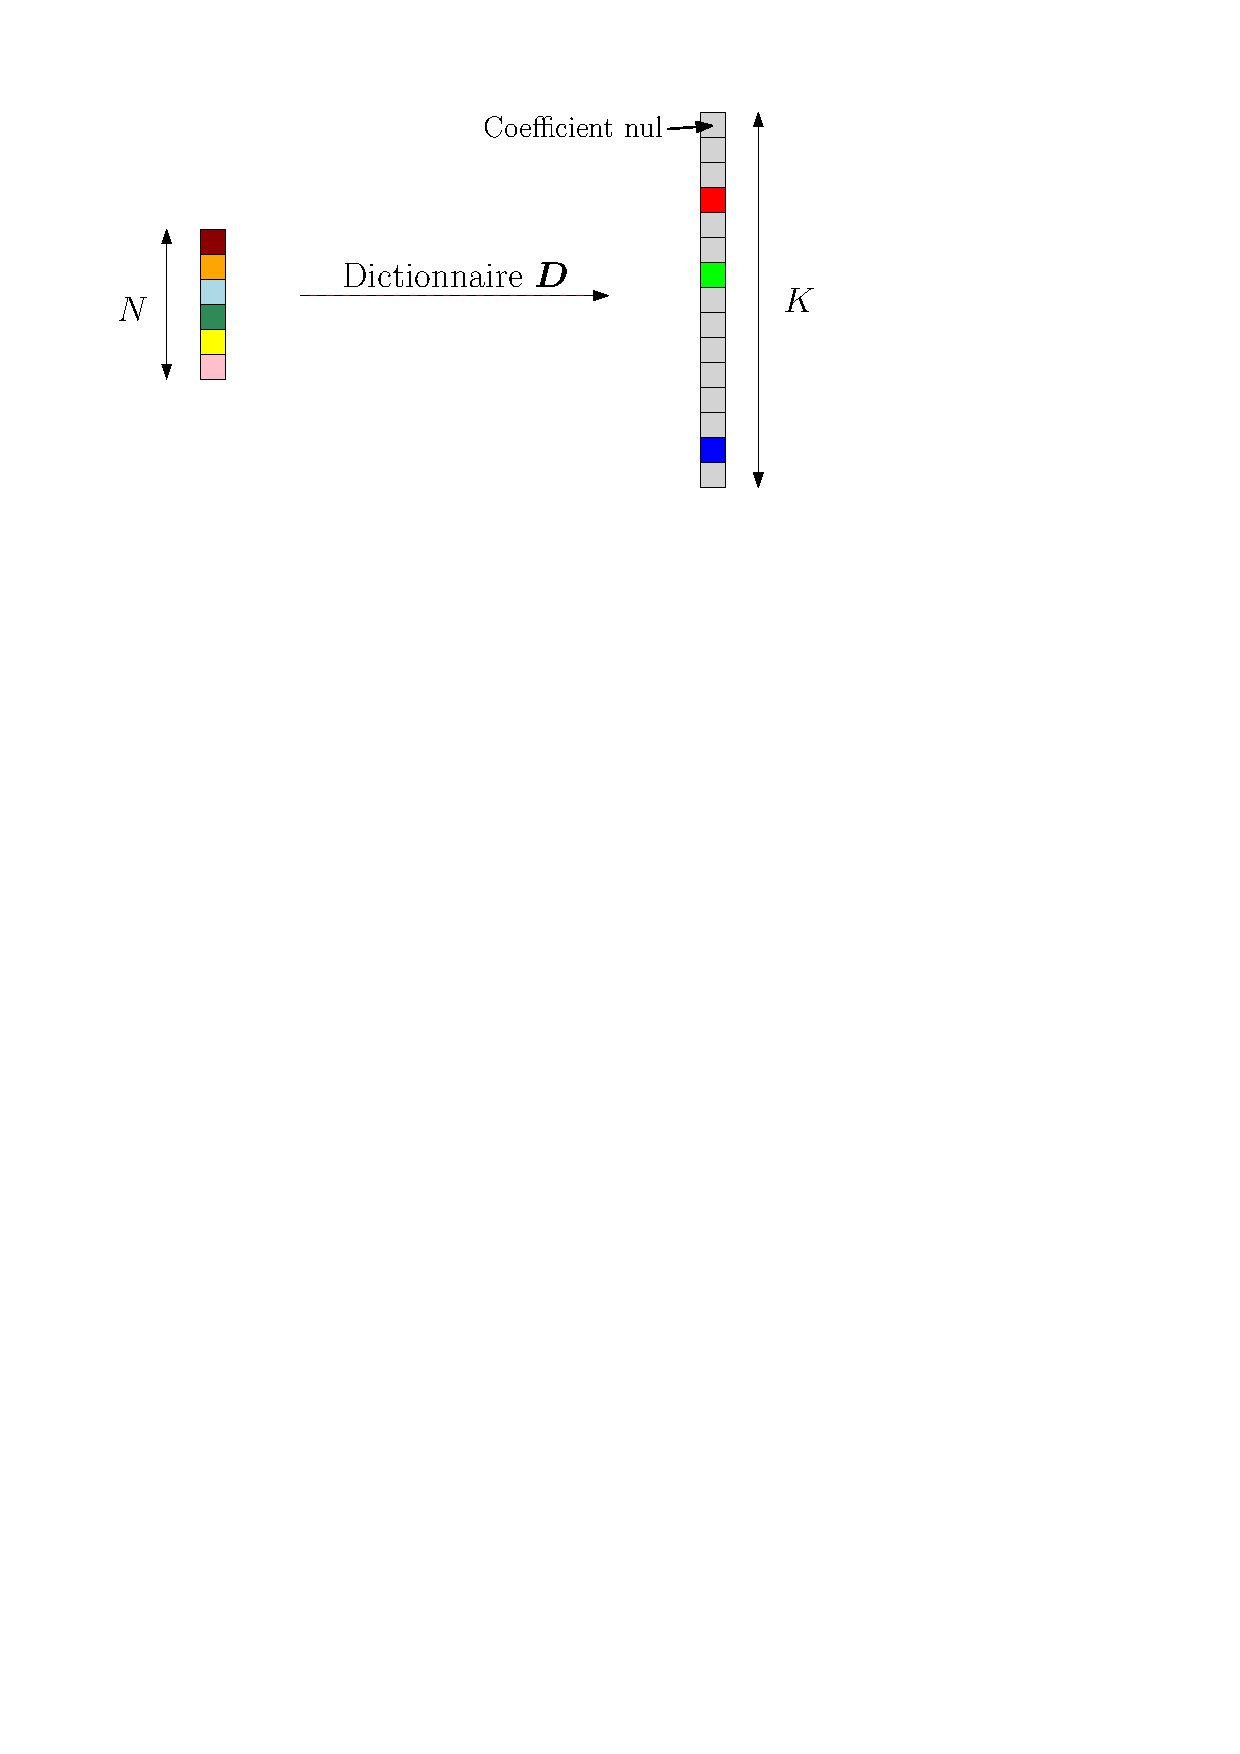
\includegraphics[width=1\linewidth]{figures/0-intro-parcimonie/representation-parcimonieuse.pdf}}
\end{figure}
\end{frame}


\begin{frame}{Exemples d'application des représentations parcimonieuses}
\begin{itemize}
\item Débruitage
	\begin{figure}\centering
	\makebox[\linewidth]{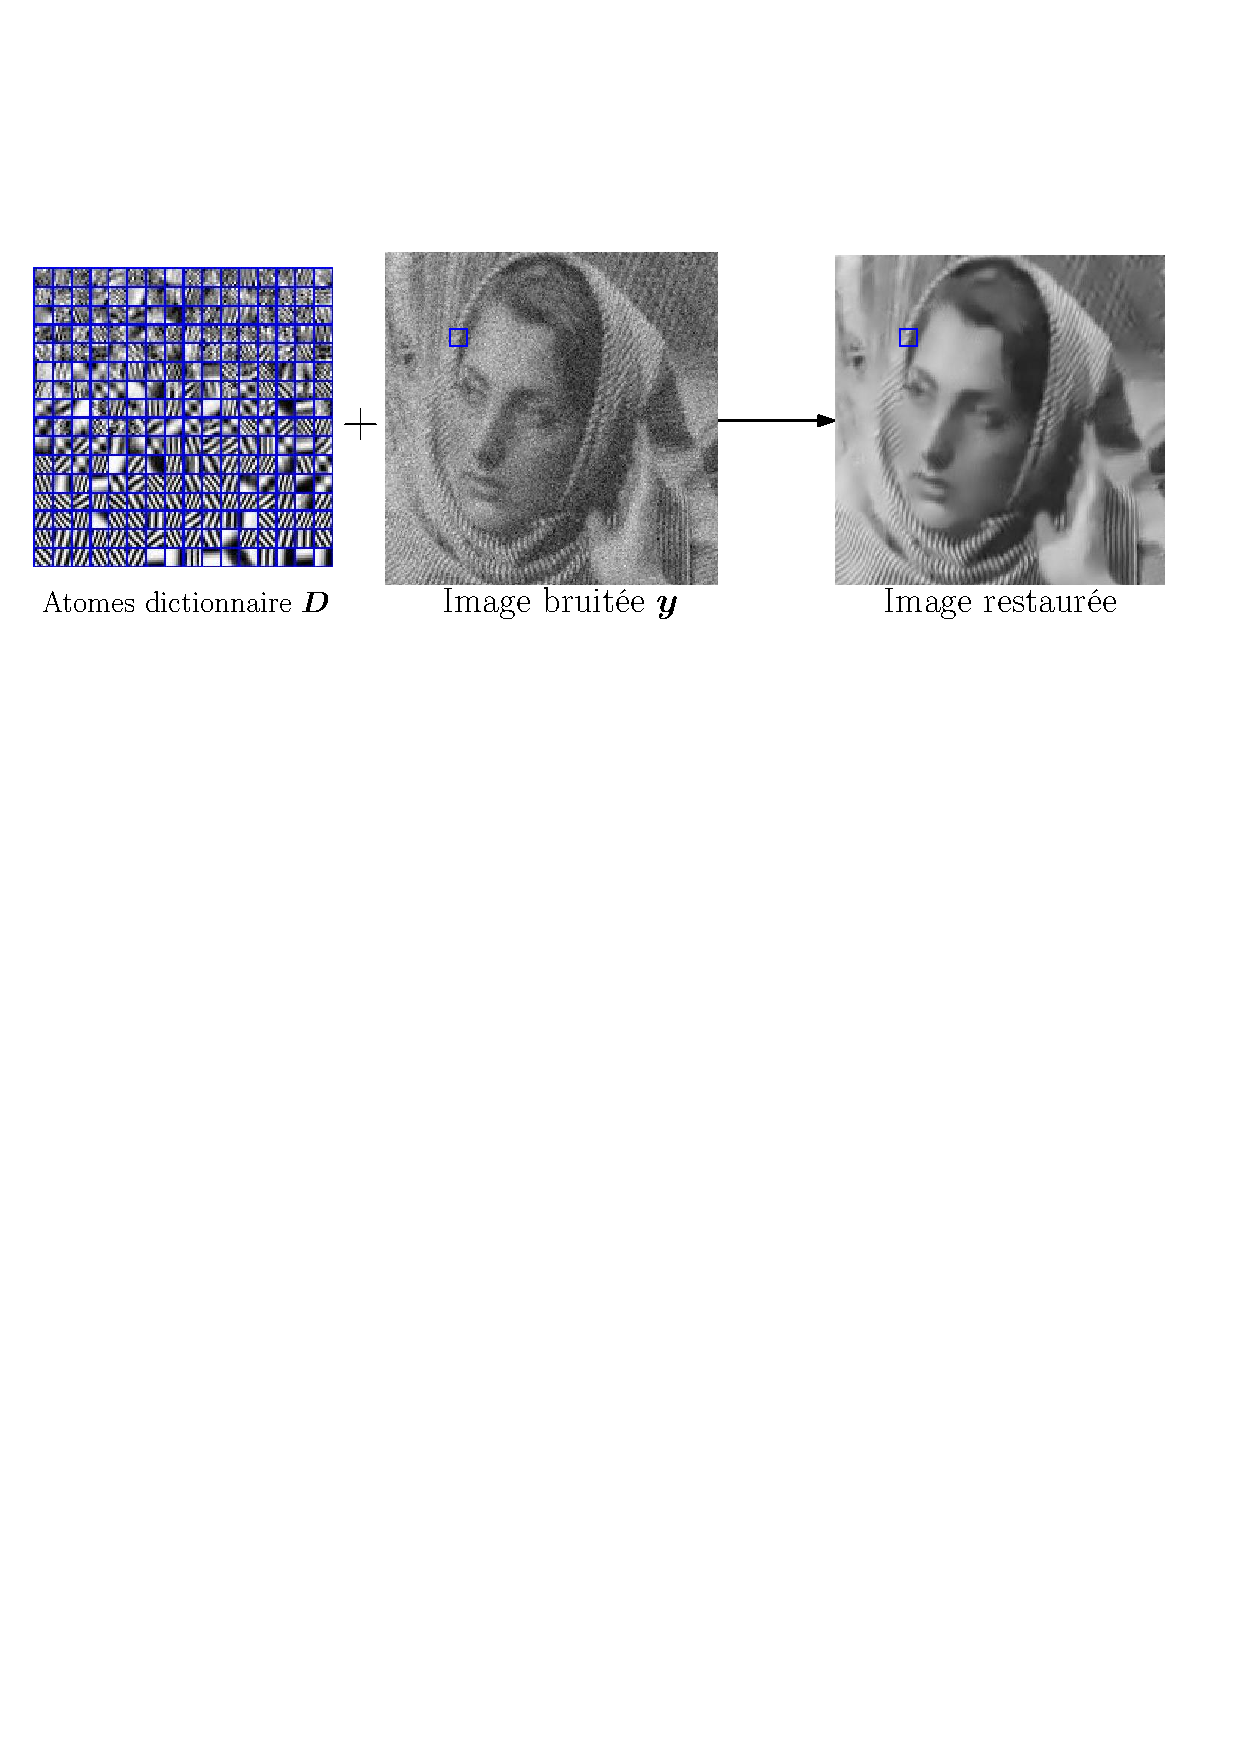
\includegraphics[width=1.1\linewidth]{figures/0-intro-parcimonie/exple-denoise.pdf}}
	\end{figure}
\item Reconnaissance d'images
\item Compression
\end{itemize}
\end{frame}


\subsection{Les dictionnaires pour la parcimonie}
\begin{frame}{Les dictionnaires pour la parcimonie}
Deux grands types de dictionnaires :
\begin{columns}[t]
\begin{column}{0.49\textwidth}
	\begin{block}{}
	Choisir un dictionnaire \alert{générique}\\
	(ondelettes, curvelets, ...)
	\begin{itemize}
	\item[\textcolor{green2}{\cmark}] transformée rapide
	\item[\textcolor{red}{\xmark}] parcimonie moyenne
	\end{itemize}
	\end{block}
\end{column}
\begin{column}{0.49\textwidth}
	\begin{block}{}
	\alert{Apprendre} le dictionnaire\\
	à partir des données
	\begin{itemize}
	\item[\textcolor{red}{\xmark}] pas de transformée rapide
	\item[\textcolor{green2}{\cmark}] parcimonie forte
	\end{itemize}
	\end{block}
	\begin{tightcenter}
		\alert{$\uparrow$}\\
		\textbf{Notre objet d'étude}
	\end{tightcenter}
\end{column}
\end{columns}


\end{frame}

\begin{frame}{Problème du coût de $\D\x$}
\vskip-3.5em
\begin{figure}\centering
\makebox[\linewidth]{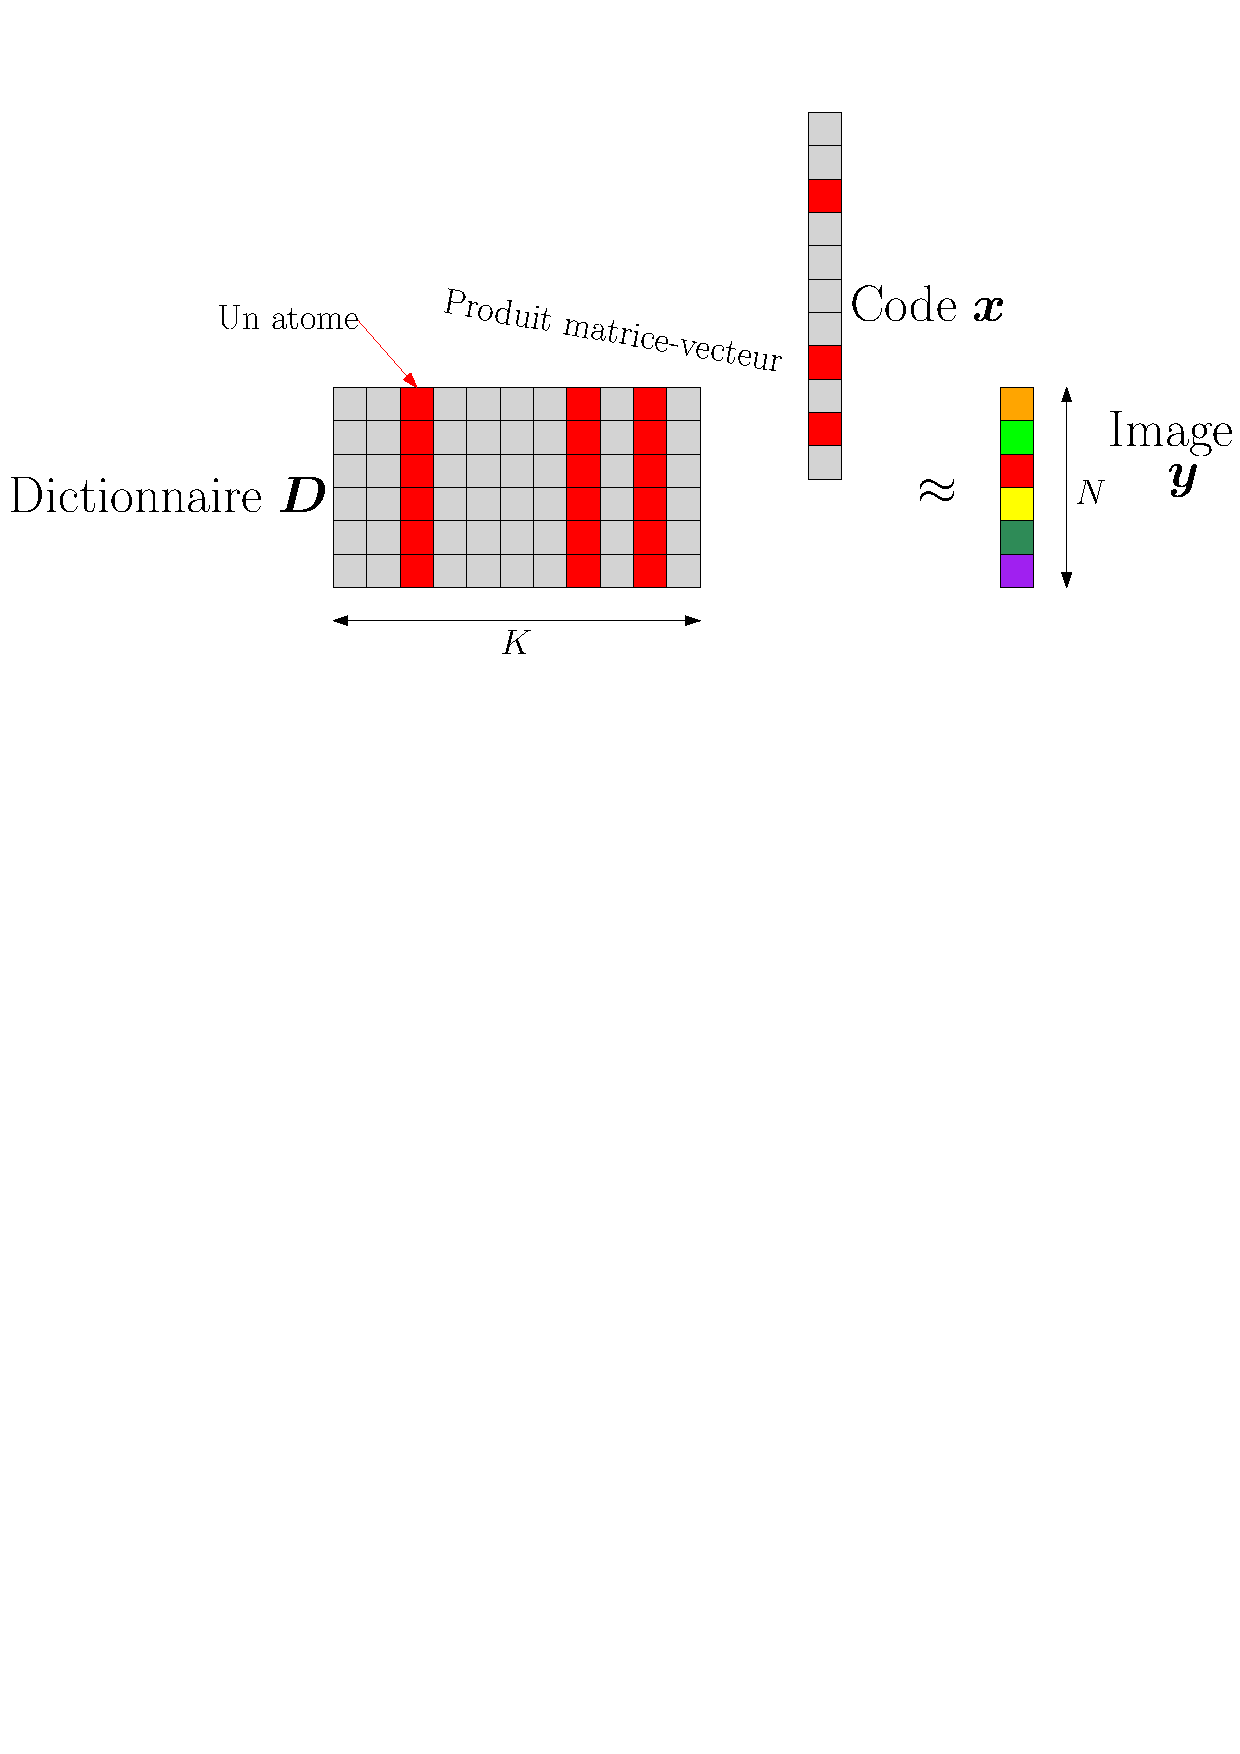
\includegraphics[width=1\linewidth]{figures/1-intro-modele/sparsity-matrix.pdf}}
\end{figure}
\vskip-0.5em
\textbf{Relaxation :} problème d'apprentissage de dictionnaire\eqref{eq_dl}
\begin{align}
\underset{\D,\x}{\min}~ & \| \x \|_1 + \lambda \| \alert{\D\x}-\y \|^2_2 \tag{$DL$}\label{eq_dl}
\end{align}

\begin{alertblock}{}
Problème : Coût élevé de \alert{$\D\x$} qui est en \alert{$O(KN)$}, $K \gg N$
\end{alertblock}
\end{frame}


\subsection{Motivations}
\begin{frame}{Motivations générales}
\begin{block}{Solution intermédiaire}
Limiter la taille des images $\rightarrow$ \alert{patches} (K-SVD)
\end{block}
\begin{itemize}
\item[\xmark] Mais on ne peut pas représenter de \alert{grandes formes}
\end{itemize}
\begin{figure}\centering
\makebox[\linewidth]{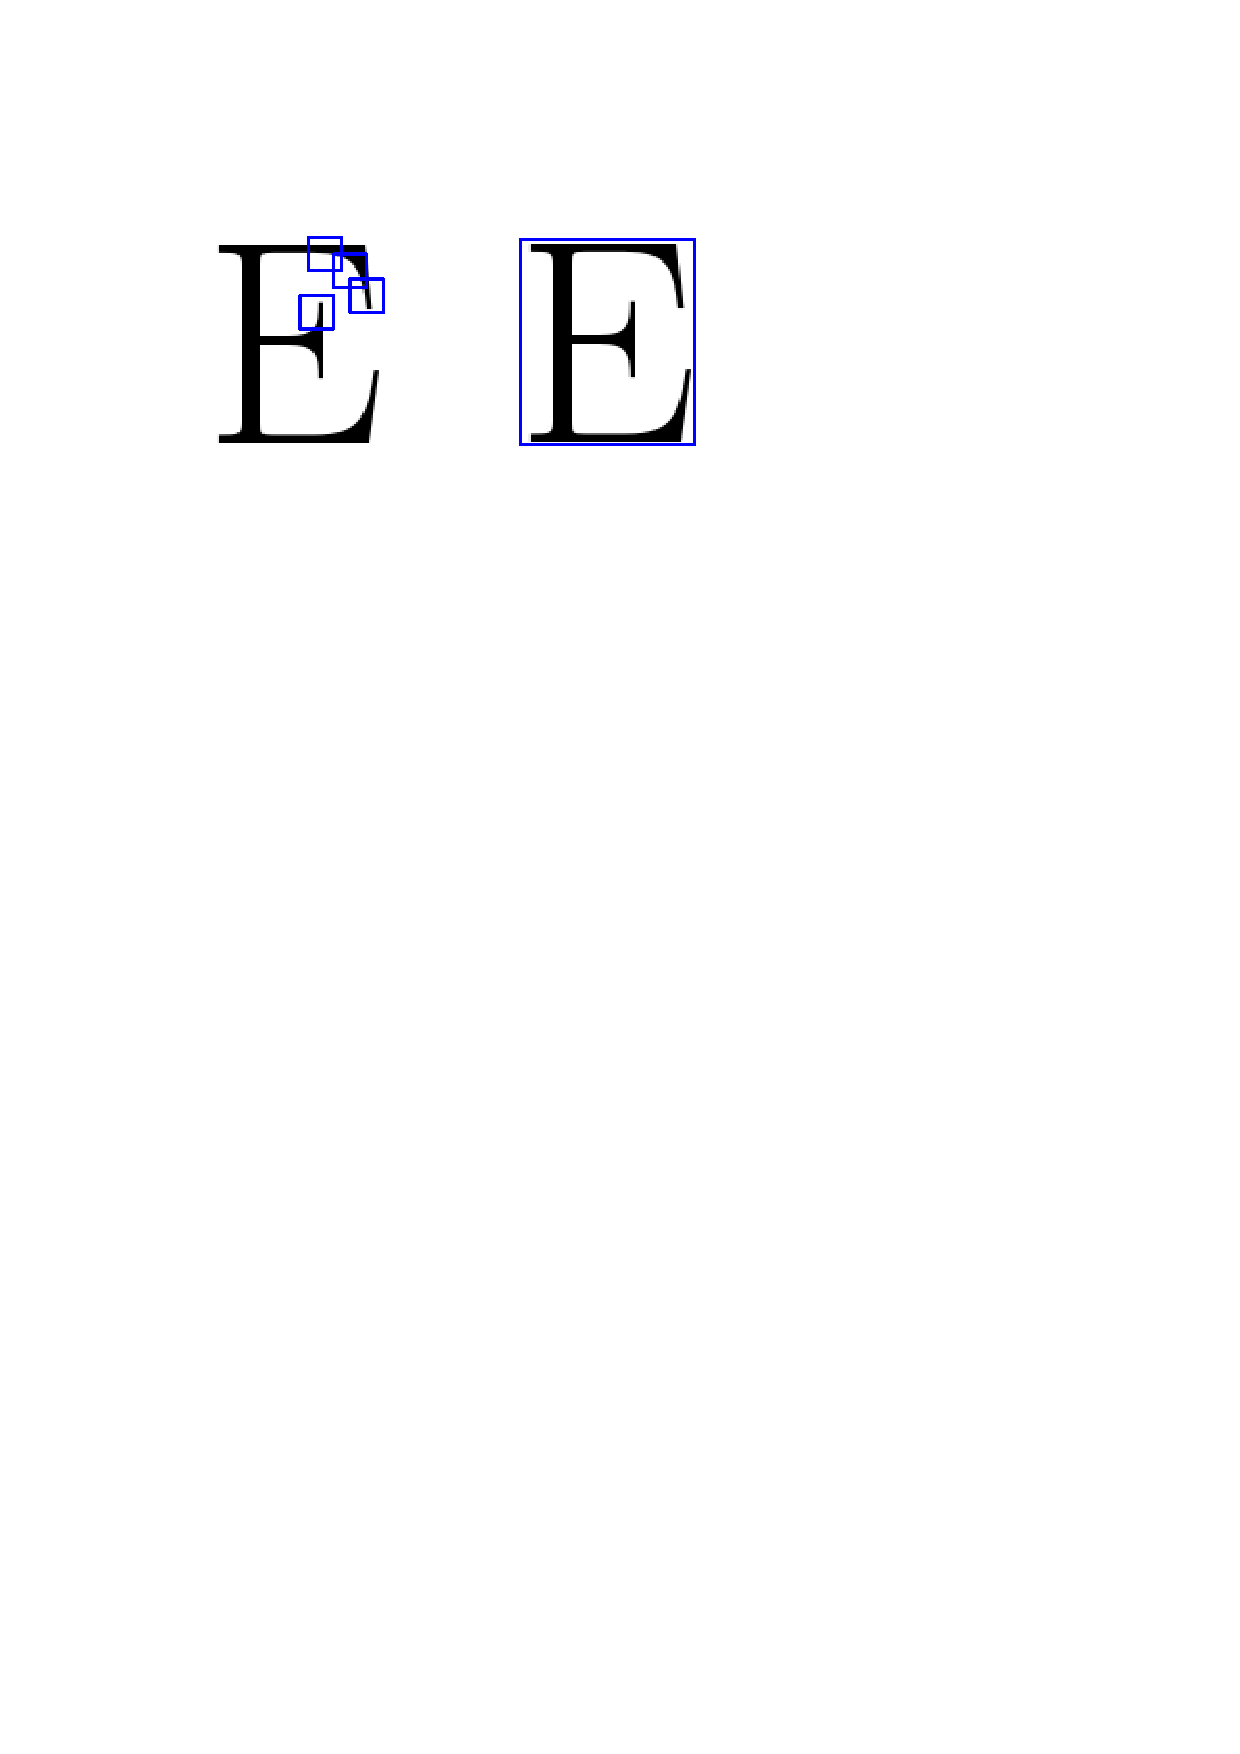
\includegraphics[width=0.5\linewidth]{figures/0-intro-parcimonie/lettre.pdf}}
\end{figure}
\begin{exampleblock}{Motivations générales}
Développer un dictionnaire \alert{appris} et \alert{rapide} adaptée aux grands atomes
\end{exampleblock}
\end{frame}







\section{État de l'art}


\subsection{Modèle d'arbre de convolutions}

\begin{frame}{Le modèle d'arbres de convolutions}
On structure le dictionnaire par un arbre de convolutions de noyaux $\h^e$ parcimonieux :
\begin{figure}\centering
\makebox[\linewidth]{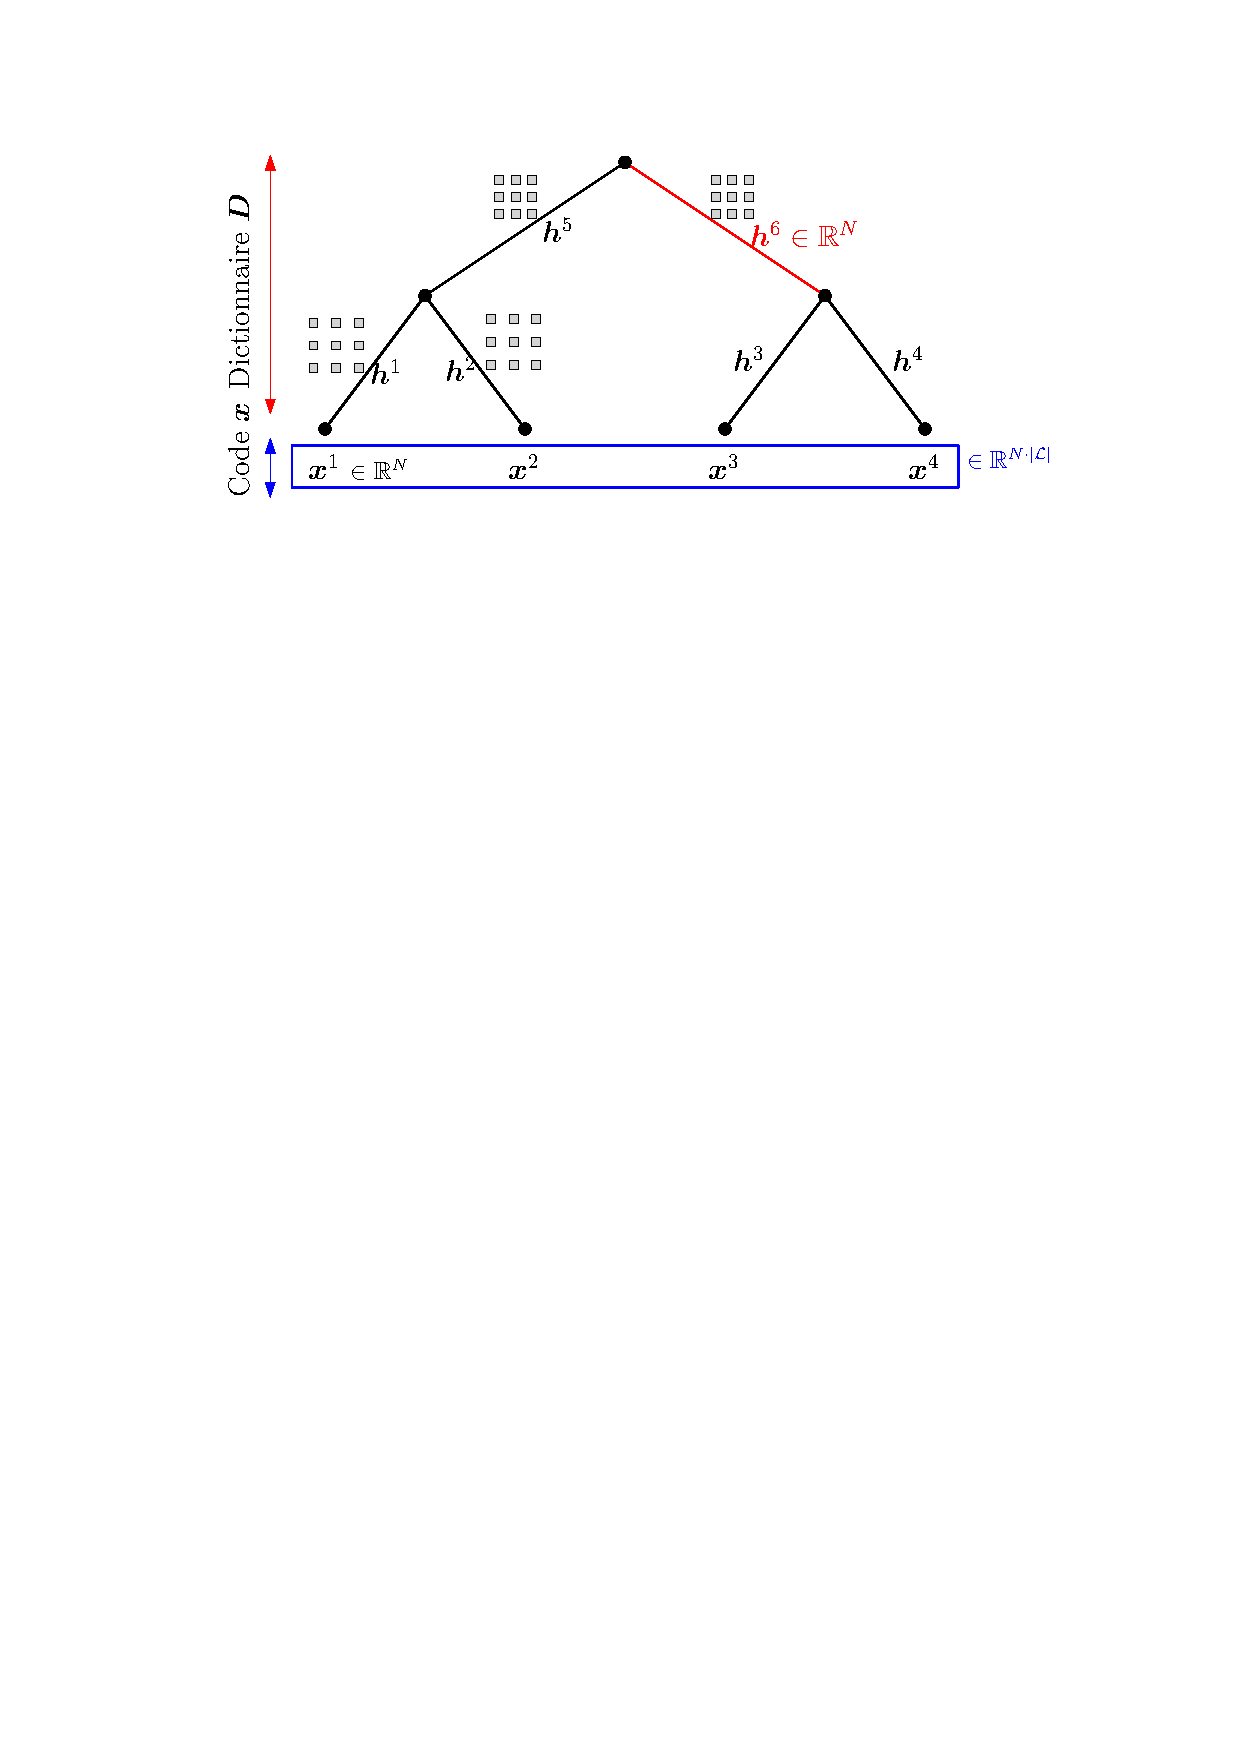
\includegraphics[width=0.8\linewidth]{figures/1-intro-modele/tree.pdf}}
\end{figure}
$\D\x$ est réduit à une complexité en \alert{$O(NQ)$} ($Q \ll N$) 
\begin{equation}
\D \x = \Beq{\sum_{l \in ~\text{Feuilles}}} \x^{\Beq{l}} * \underbrace{\h^{\Beq{l}}* \dots* \h^{r}}_{\textrm{de la racine à la feuille}}
\end{equation}
{\small (Q est le nombre total d'éléments des supports des noyaux)}
\end{frame}
 

\begin{frame}{Problème associé}
On appelle (${FTL}$) (\emph{Fast Transform Learning}) l'adaptation de \eqref{eq_dl} à ce modèle :

\begin{columns}
	

\begin{column}{0.7\linewidth}
\begin{equation*}
\tag{${FTL}$} \min_{\substack{(\h^e)_{e \in \E} \\ \h^e \in \Dspace^e}}
	\underbrace{\norm{\Beq{\sum_{l \in Feuilles}} \x^{\Beq{l}} * \h^{*\Beq{l}} -\y}{2}^2}_{\text{Fonction objectif } \alert{E(\h)}}  \label{eq_ftl} \notag
\end{equation*}
\end{column}
\begin{column}{0.3\linewidth}
\begin{itemize}
	\item[\xmark] non-convexe
	\item[\cmark] mais convexe marginalement
\end{itemize}
\end{column}
\end{columns}
avec $\Dspace^e$ la contrainte sur les supports des noyaux $\h^e$.

L'algorithme \alert{PALMTREE} donne une solution approchée :
\begin{itemize}
	\item \cite{bolte_proximal_2014} : Basé sur PALM (descente de gradient proximal alterné)
	\item \cite{chabiron_toward_2015} : \eqref{eq_ftl} vérifie les hypothèse de convergence pour PALM
	\item \cite{chabiron_optimization_2016} : le point  critique atteint n'est pas trop éloigné du minimum global
\end{itemize}
\end{frame}

\subsection{L'algorithme PALMTREE}
\begin{frame}{Exemple de solution de PALMTREE}
Données en entrée de PALMTREE
\begin{itemize}
	\item image $\y$,
	\item code $\x$ \alert{fixé} (un code $\x^l \in \R^N$ par feuille)
	\item supports $\s^e$, arbre $\T$
\end{itemize}
\begin{figure}\centering
\makebox[\linewidth]{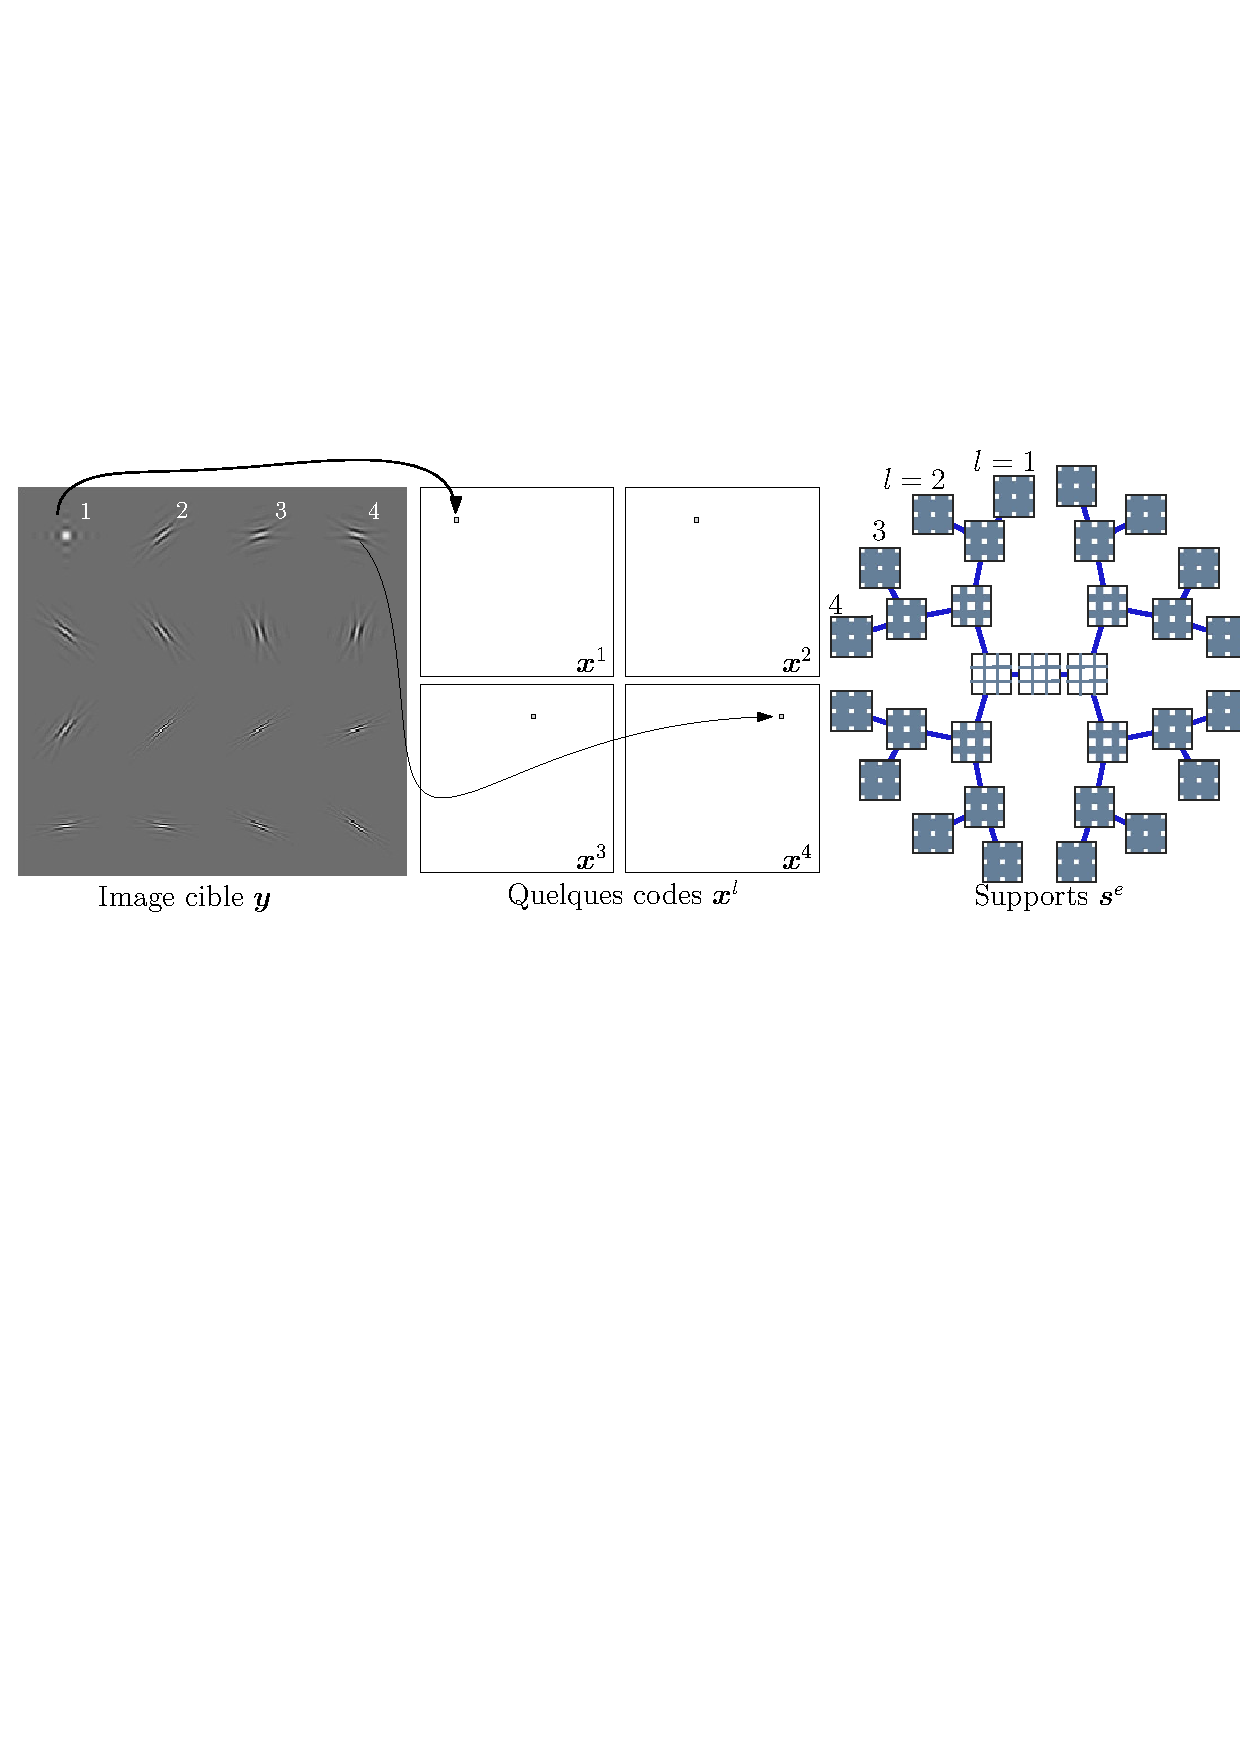
\includegraphics[width=1.1\linewidth]{figures/1-intro-modele/intro-inputs.pdf}}
\end{figure}
\end{frame}


\begin{frame}{Exemple de solution de PALMTREE}
Données en sortie de PALMTREE
\begin{itemize}
	\item les \alert{noyaux} $\h$ (on note $\h = (\h^e)_{e \in \E}$)
\end{itemize}
\begin{figure}\centering
\makebox[\linewidth]{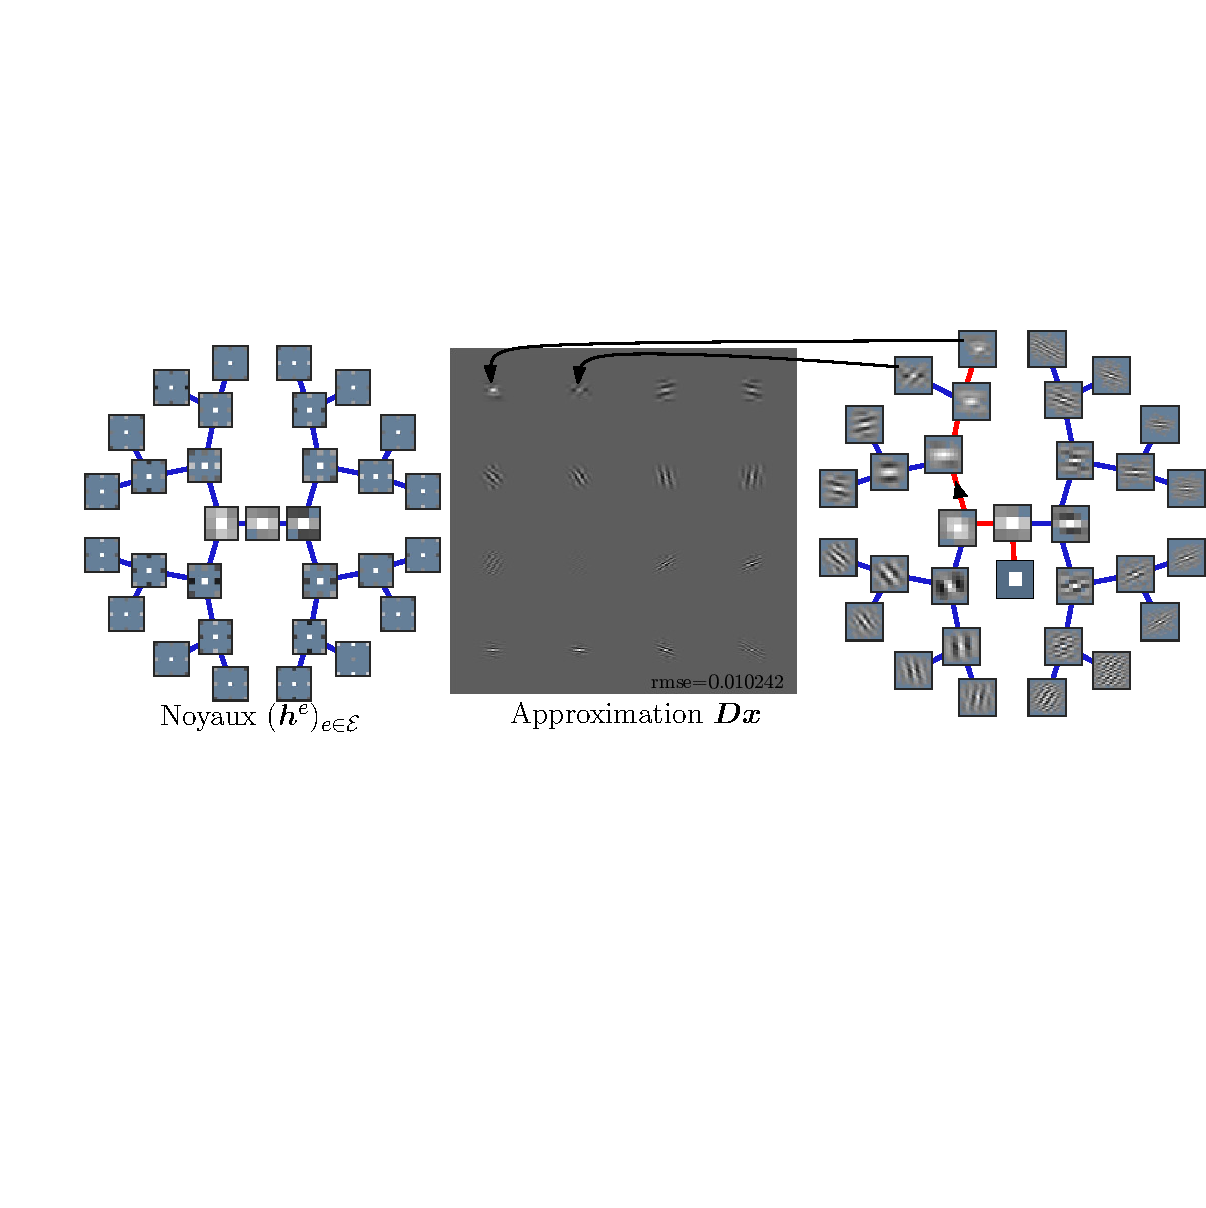
\includegraphics[width=1.1\linewidth]{figures/1-intro-modele/intro-outputs.pdf}}
\end{figure}
\end{frame}


\subsection{Objectifs du stage}
\begin{frame}{Objectifs du stage}
\begin{figure}\centering
    \makebox[\linewidth]{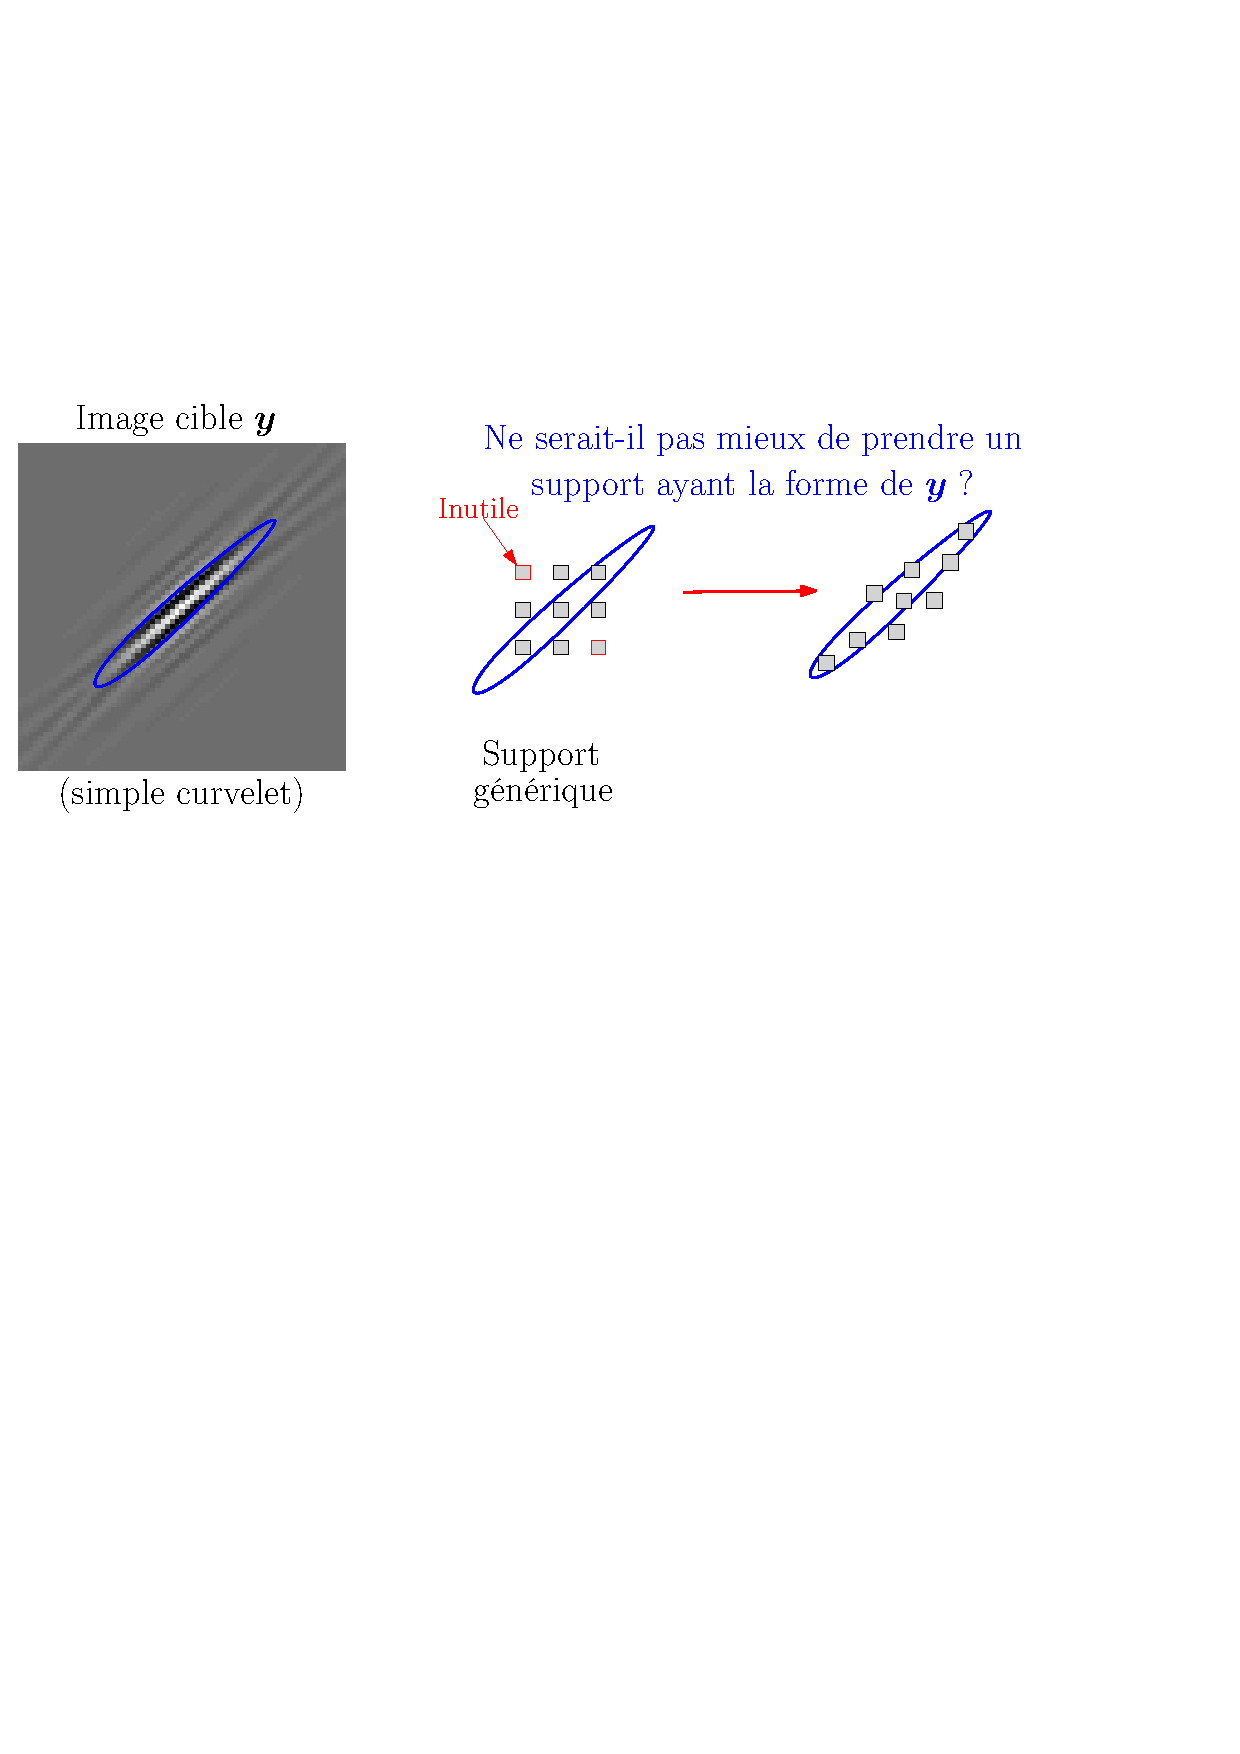
\includegraphics[width=1\linewidth]{figures/0-intro-parcimonie/meilleur-support.pdf}}
\end{figure}
\begin{alertblock}{Inconvénients de PALMTREE}\centering
\begin{itemize}
\item Supports des noyaux \alert{fixes} $\rightarrow$ perte d'adaptabilité
\end{itemize}
\end{alertblock}
\begin{exampleblock}{Objectifs du stage} \centering
Estimer les supports des noyaux à partir de l'image $\y$
\end{exampleblock}
\end{frame}




\section{Travail réalisé}

\subsection{Idée directrice inspirée de l'OMP}
\begin{frame}{L'idée}
\begin{block}{Algorithme OMP (Orthogonal Matching Pursuit)}
	\begin{enumerate}
		\item \textbf{Chercher} élément à ajouter au support $\rightarrow$ \alert{gradient $\nabla E(\H)$}
		\item \textbf{Recalculer} les noyaux $\rightarrow$ \alert{PALMTREE}
		\item Recommencer
	\end{enumerate}
\end{block}
\begin{exampleblock}{Questions}
\begin{enumerate}
	\item Gradient adapté pour ajouter le meilleur élément possible ?
	\item Cet algorithme fonctionne t-il dans le cadre d'un arbre ?
\end{enumerate}
\end{exampleblock}
\end{frame}


\subsection{Gradient adapté pour ajouter des éléments ?}

\begin{frame}{Explications des expériences sur le gradient}
\alert{Données en entrée} de PALMTREE pour les expériences sur le gradient
\begin{figure}\centering
    \makebox[\linewidth]{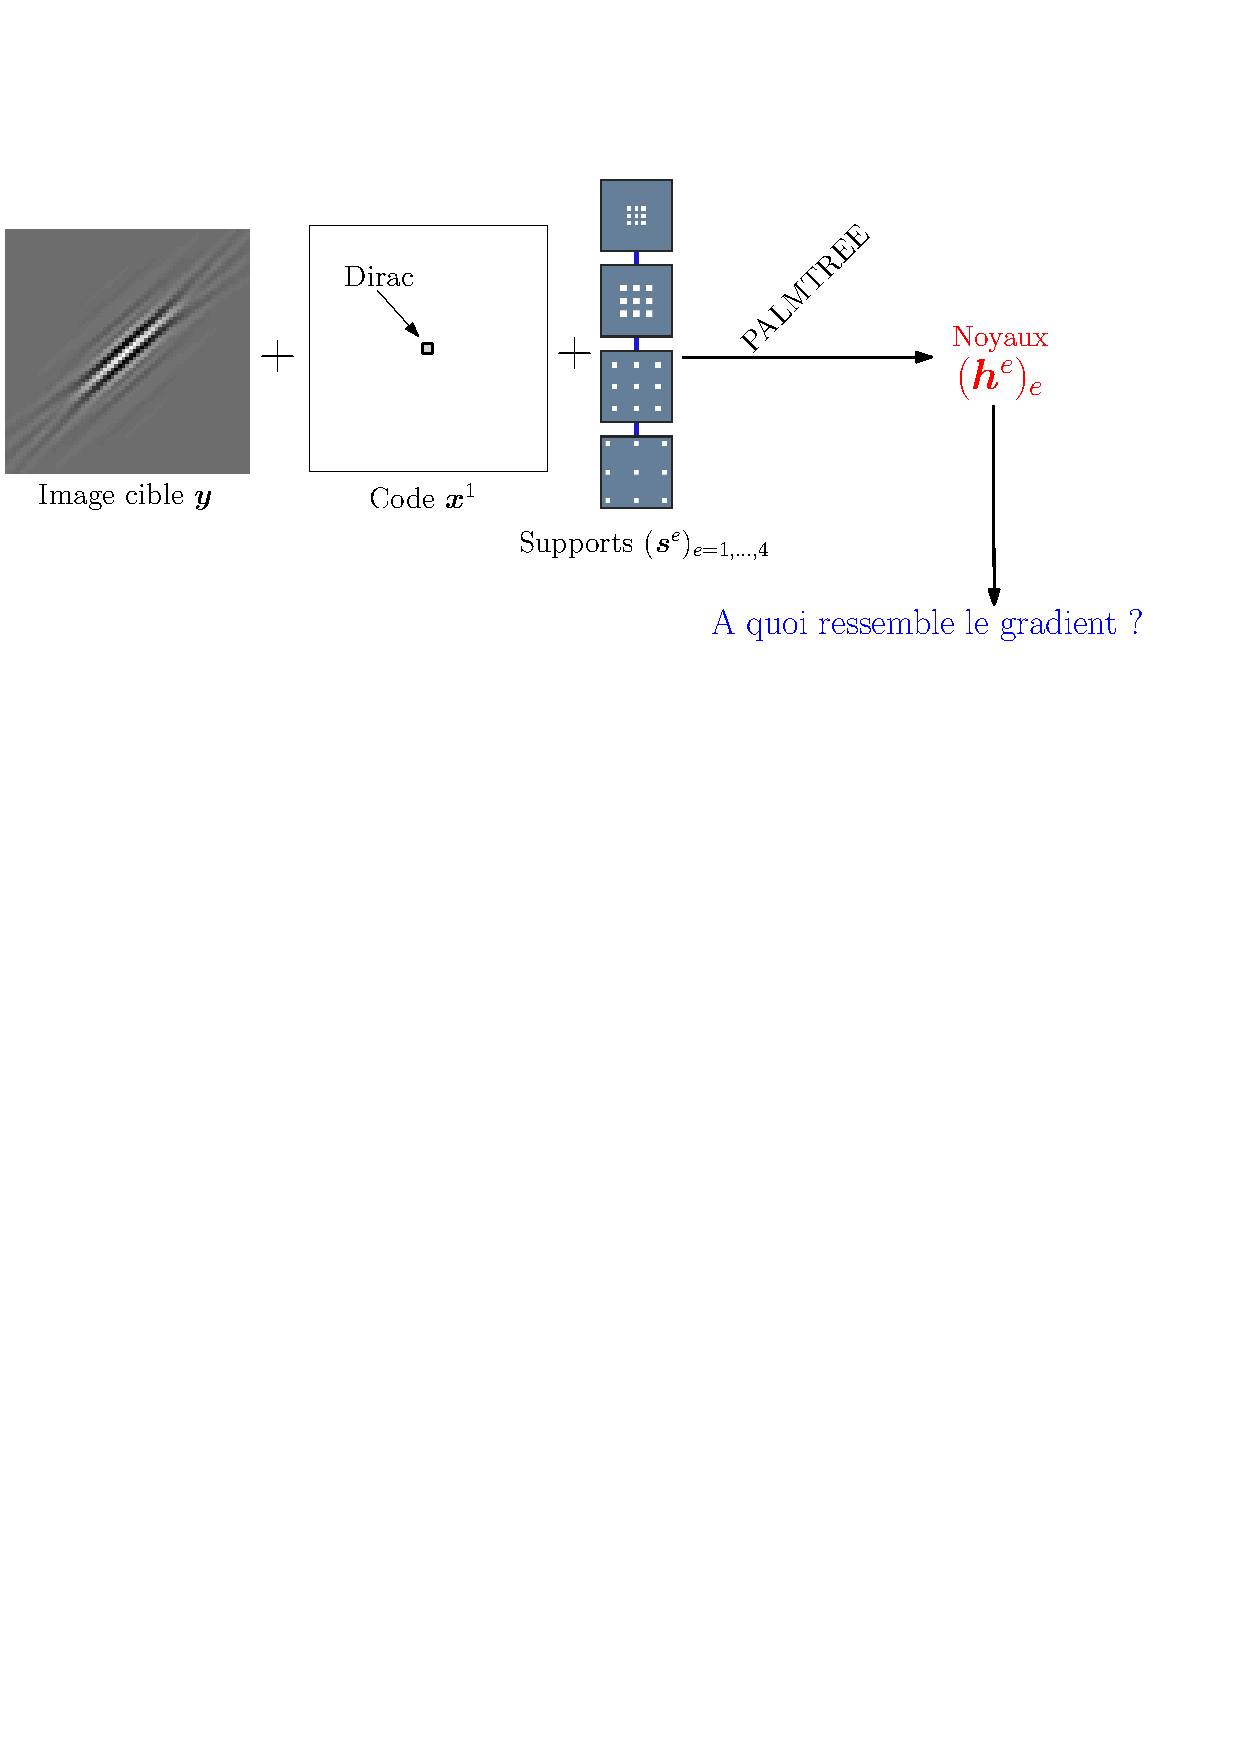
\includegraphics[width=1\linewidth]{figures/2-check-gradient/branche-setup.pdf}}
\end{figure}
\end{frame}

\begin{frame}{Gain versus gradient}
\begin{figure}\centering
    \makebox[\linewidth]{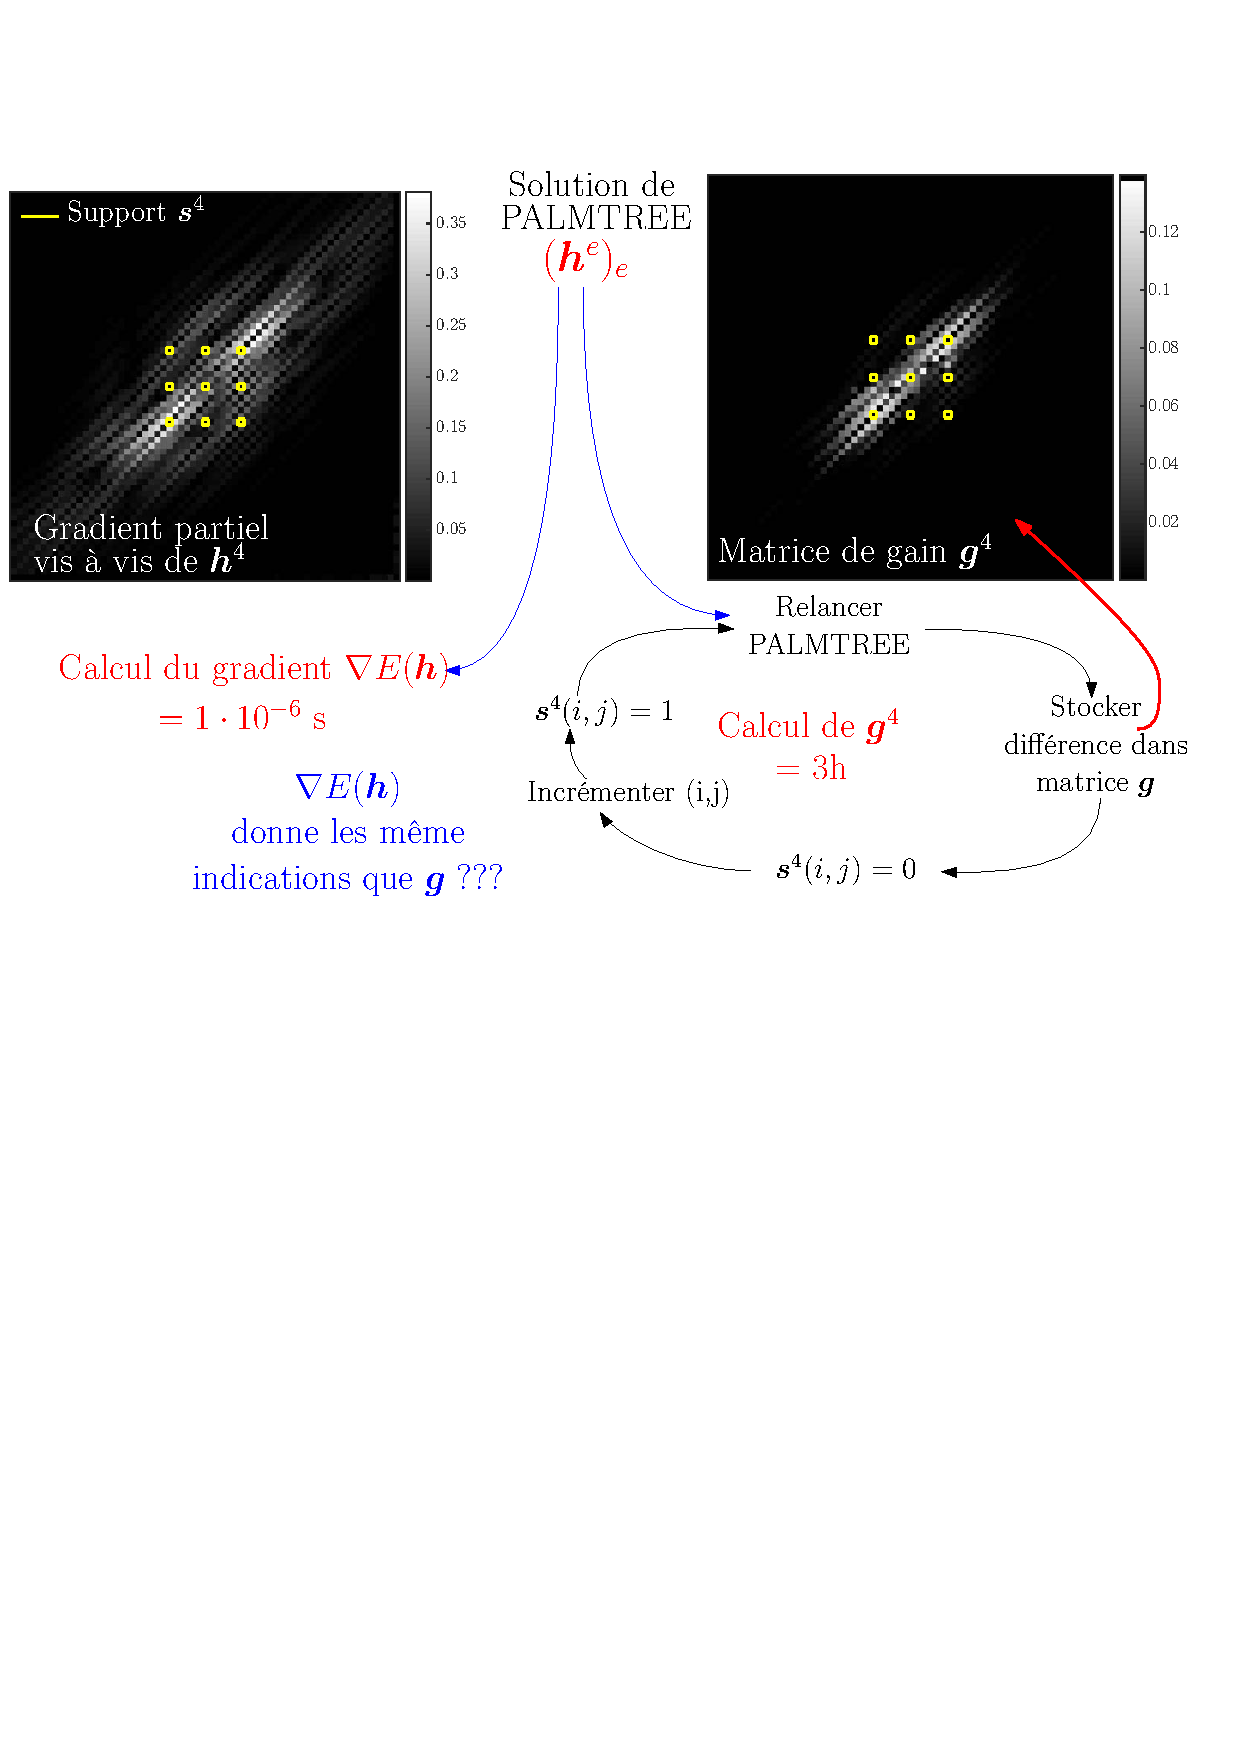
\includegraphics[width=1.1\linewidth]{figures/2-check-gradient/gradient-vs-gain.pdf}}
\end{figure}
\end{frame}

\begin{frame}{Résultats après ajout}
\begin{figure}\centering
    \makebox[\linewidth]{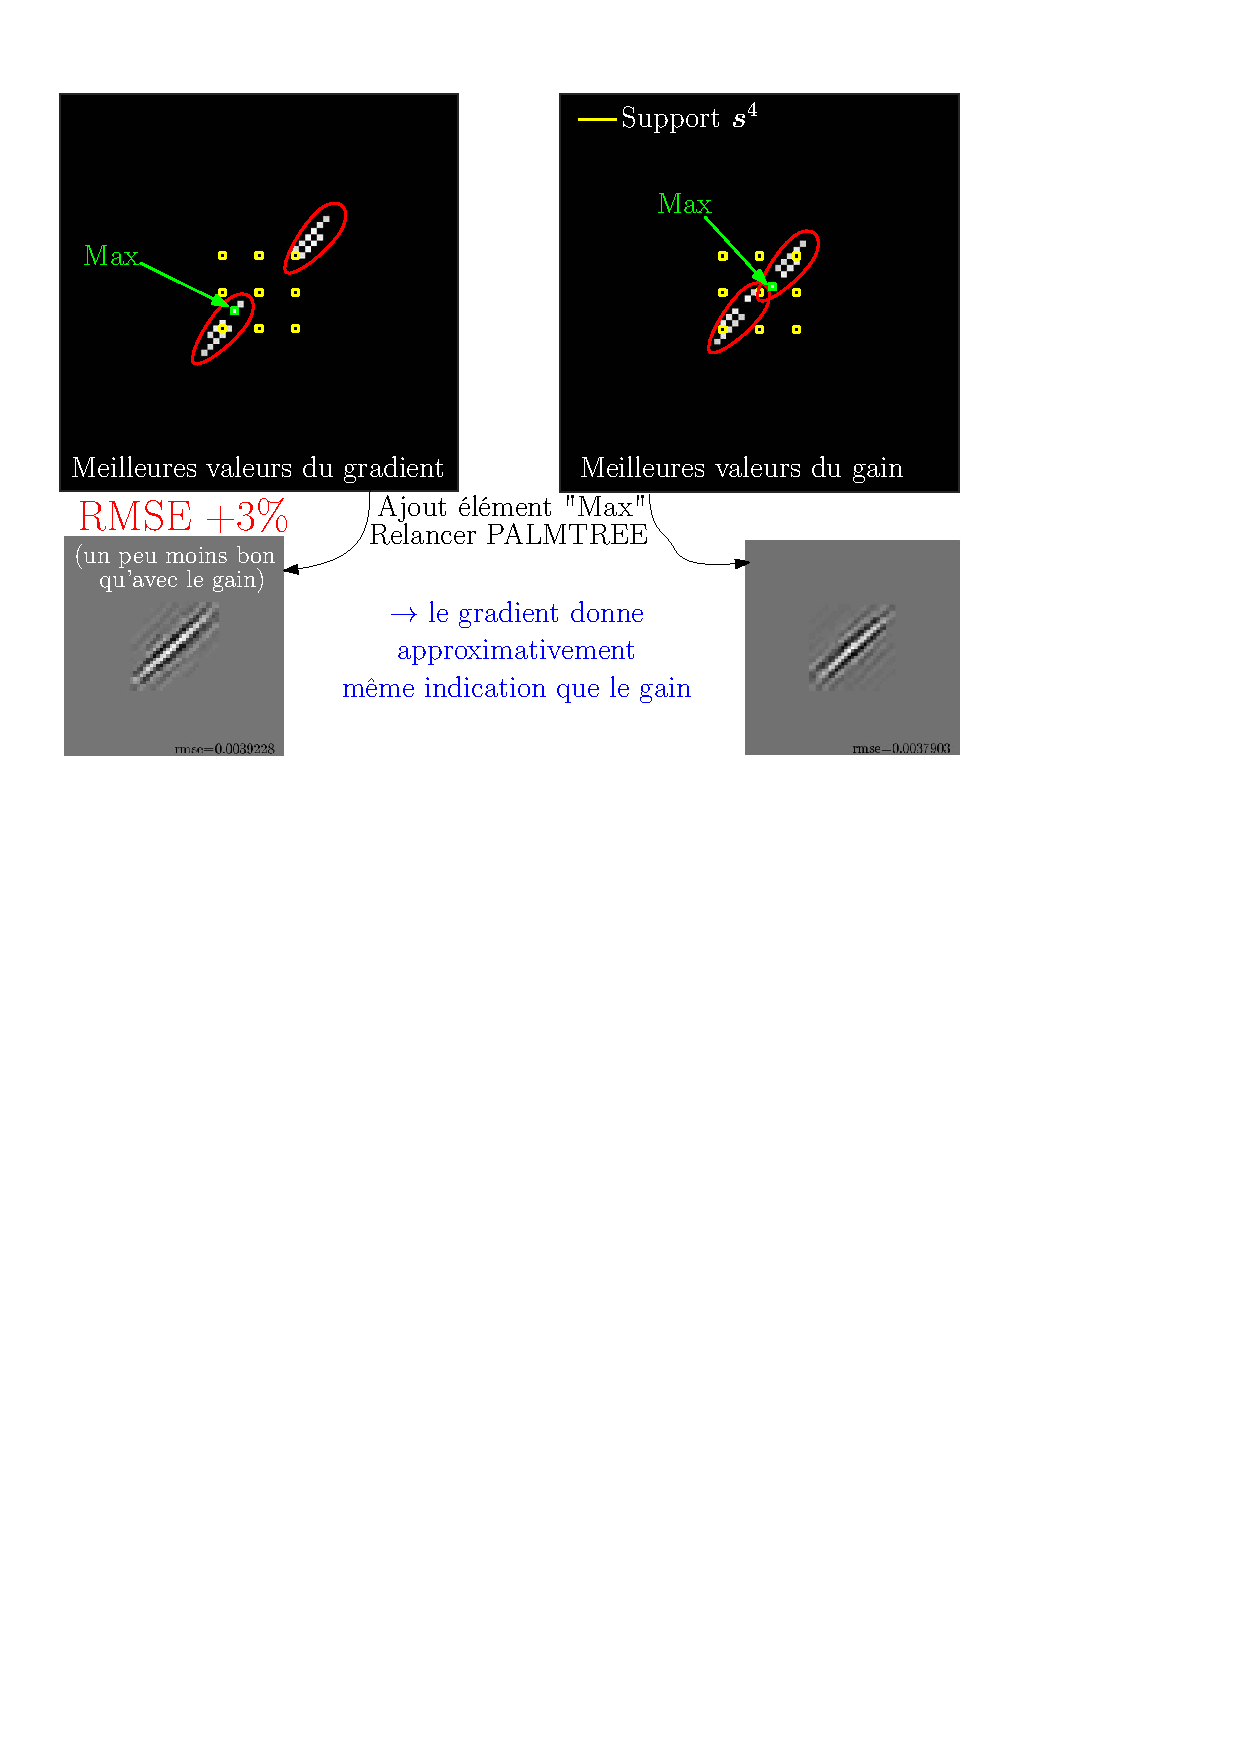
\includegraphics[width=1.0\linewidth]{figures/2-check-gradient/apres-ajout.pdf}}
\end{figure}
\end{frame}

\subsection{Ça fonctionne sur un arbre ?}

\begin{frame}{Explication des expériences sur un arbre}
\alert{Données en entrée} pour les expériences sur les arbres
\begin{figure}\centering
    \makebox[\linewidth]{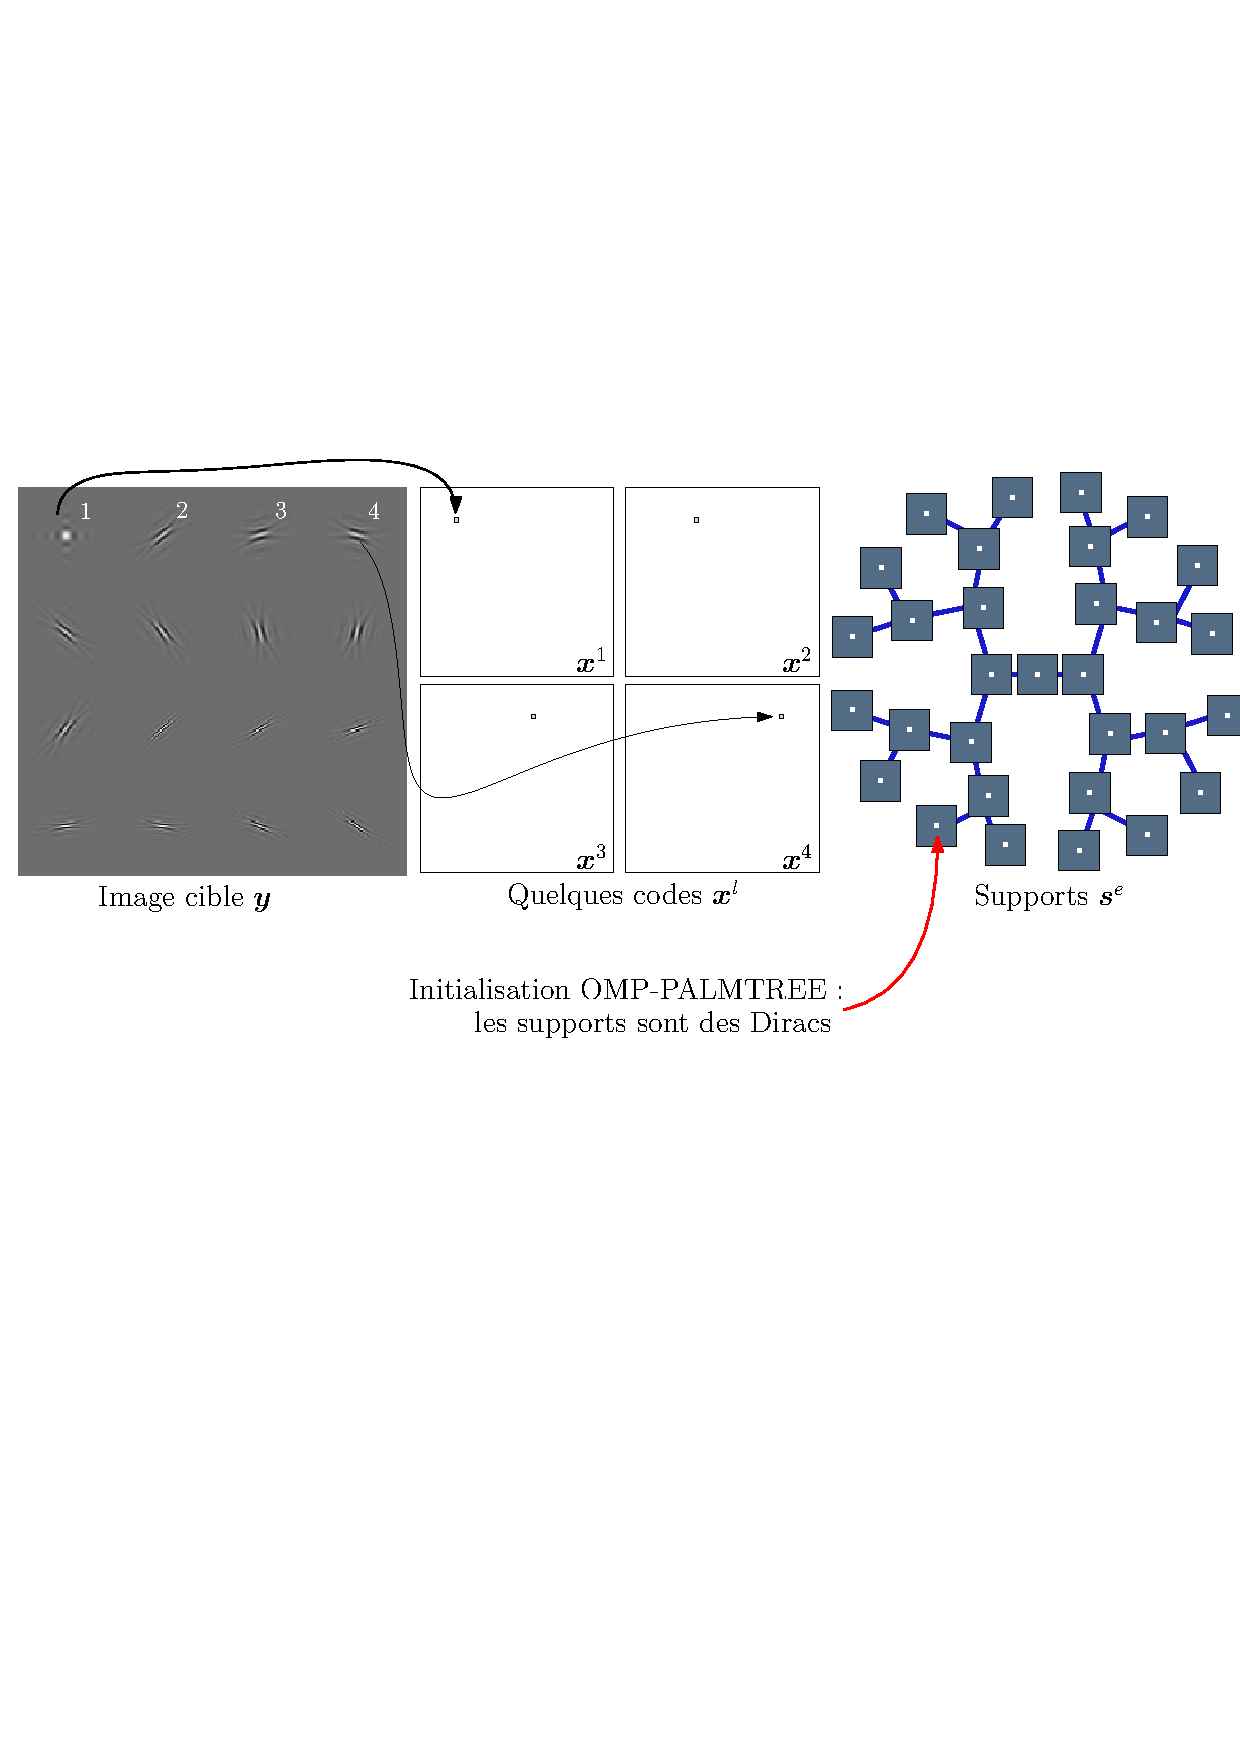
\includegraphics[width=1.0\linewidth]{figures/3-learn-tree-scattered/learn-inputs.pdf}}
\end{figure}
\end{frame}

\begin{frame}{Détail algorithme OMP-PALMTREE}
\begin{figure}\centering
    \makebox[\linewidth]{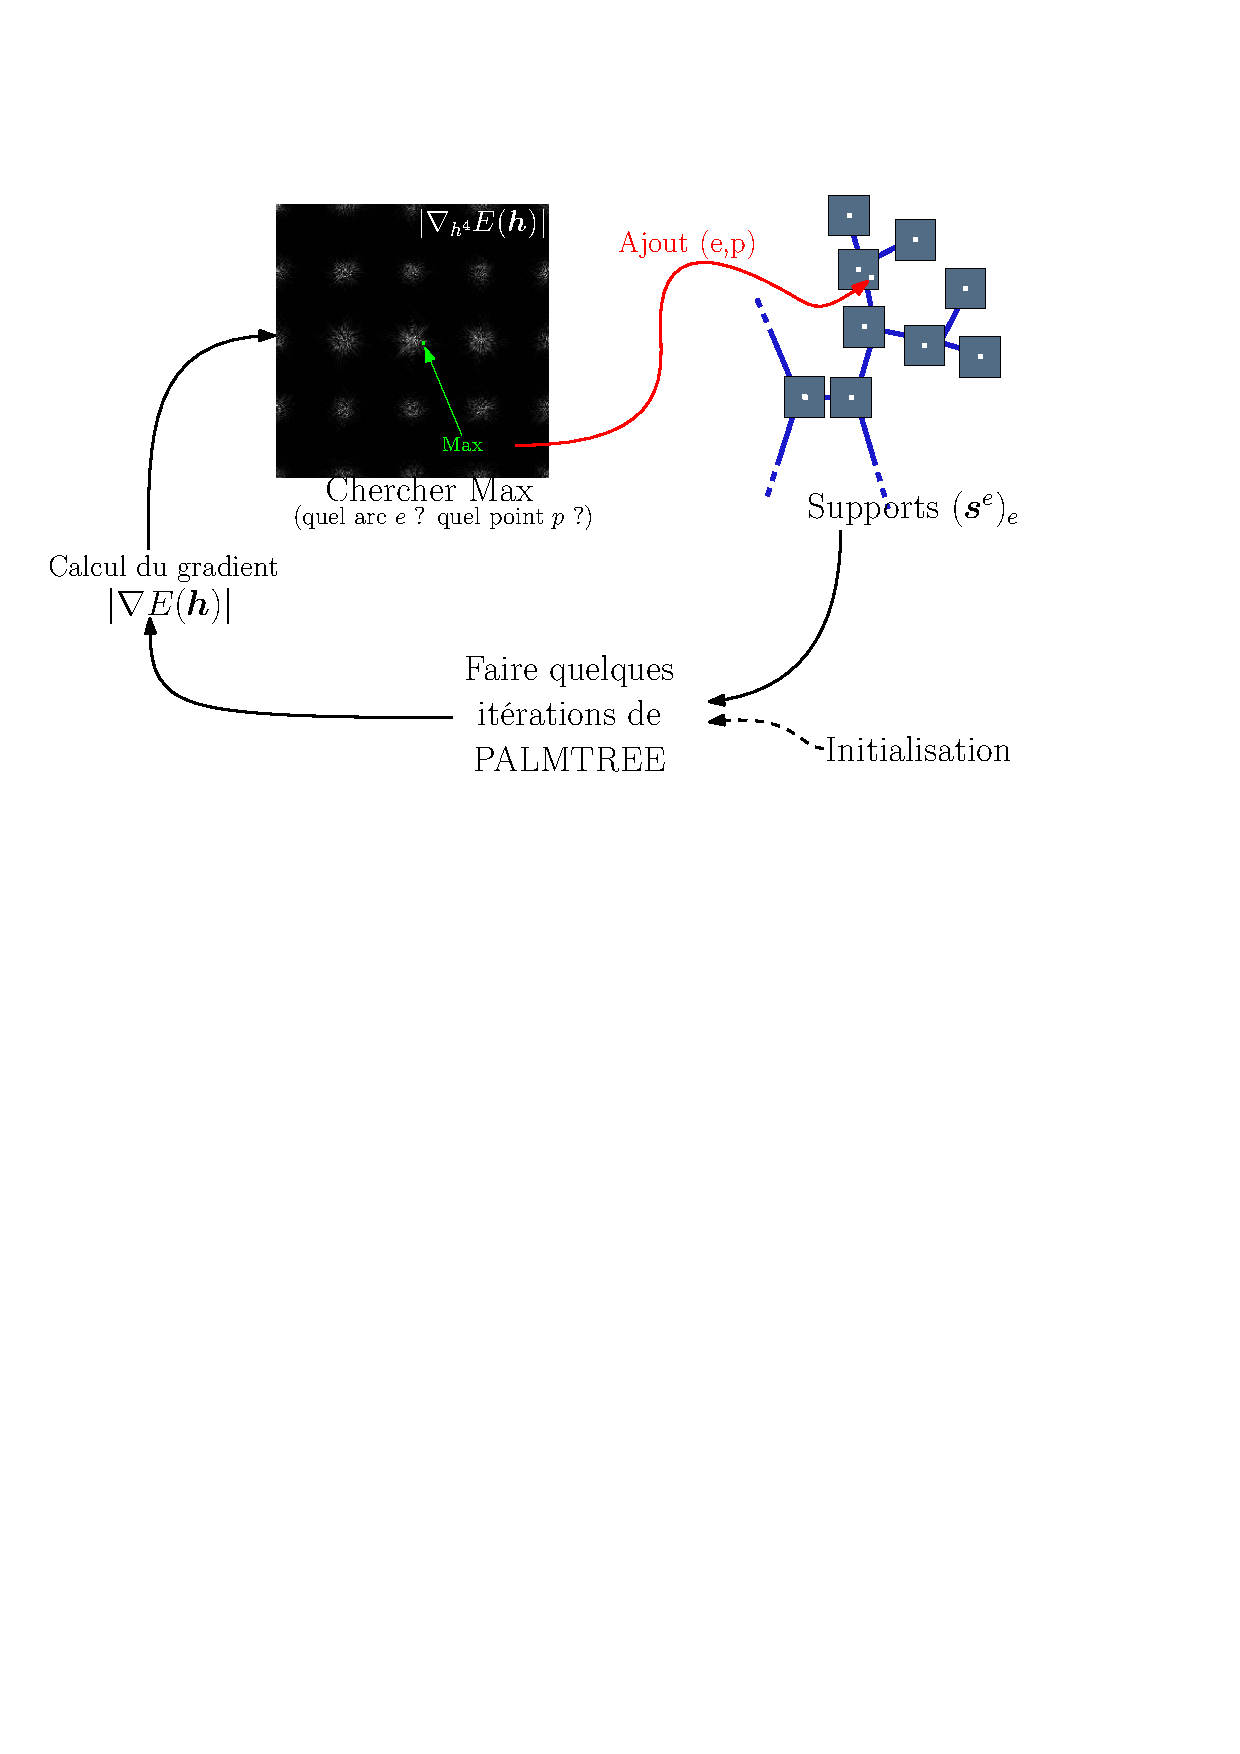
\includegraphics[width=1.1\linewidth]{figures/3-learn-tree-scattered/algo-omp-palmtree.pdf}}
\end{figure}
\end{frame}

\begin{frame}{Problème des supports dispersés}
\begin{figure}\centering
    \makebox[\linewidth]{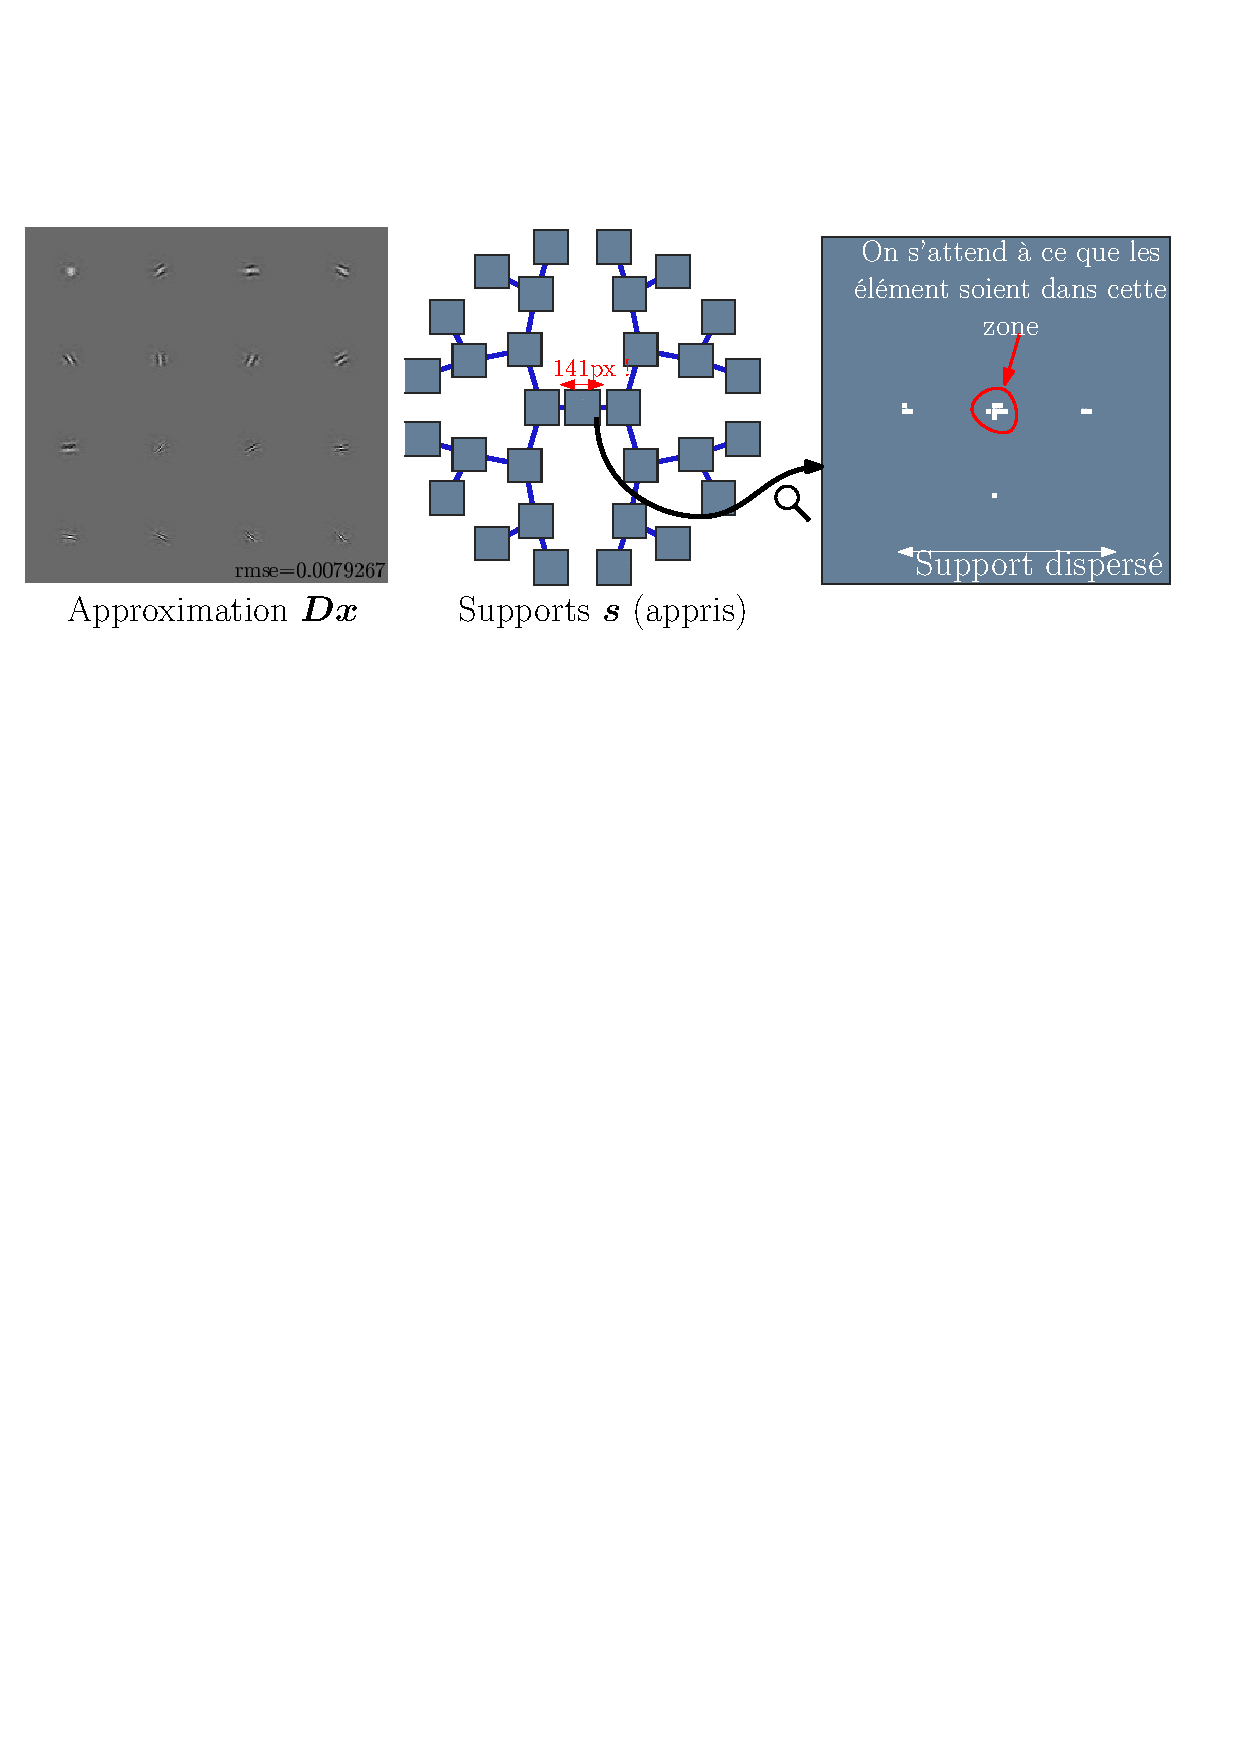
\includegraphics[width=1.1\linewidth]{figures/3-learn-tree-scattered/scattered-tree.pdf}}
\end{figure}
\begin{alertblock}{Problème d'identifiabilité des atomes}\centering
16 \alert{grands} atomes interdépendants \textbf{ou} 16 \alert{petits} atomes bien localisés ?
\end{alertblock}
\end{frame}

\begin{frame}{Ajout d'un à priori sur les supports}
\begin{figure}\centering
    \makebox[\linewidth]{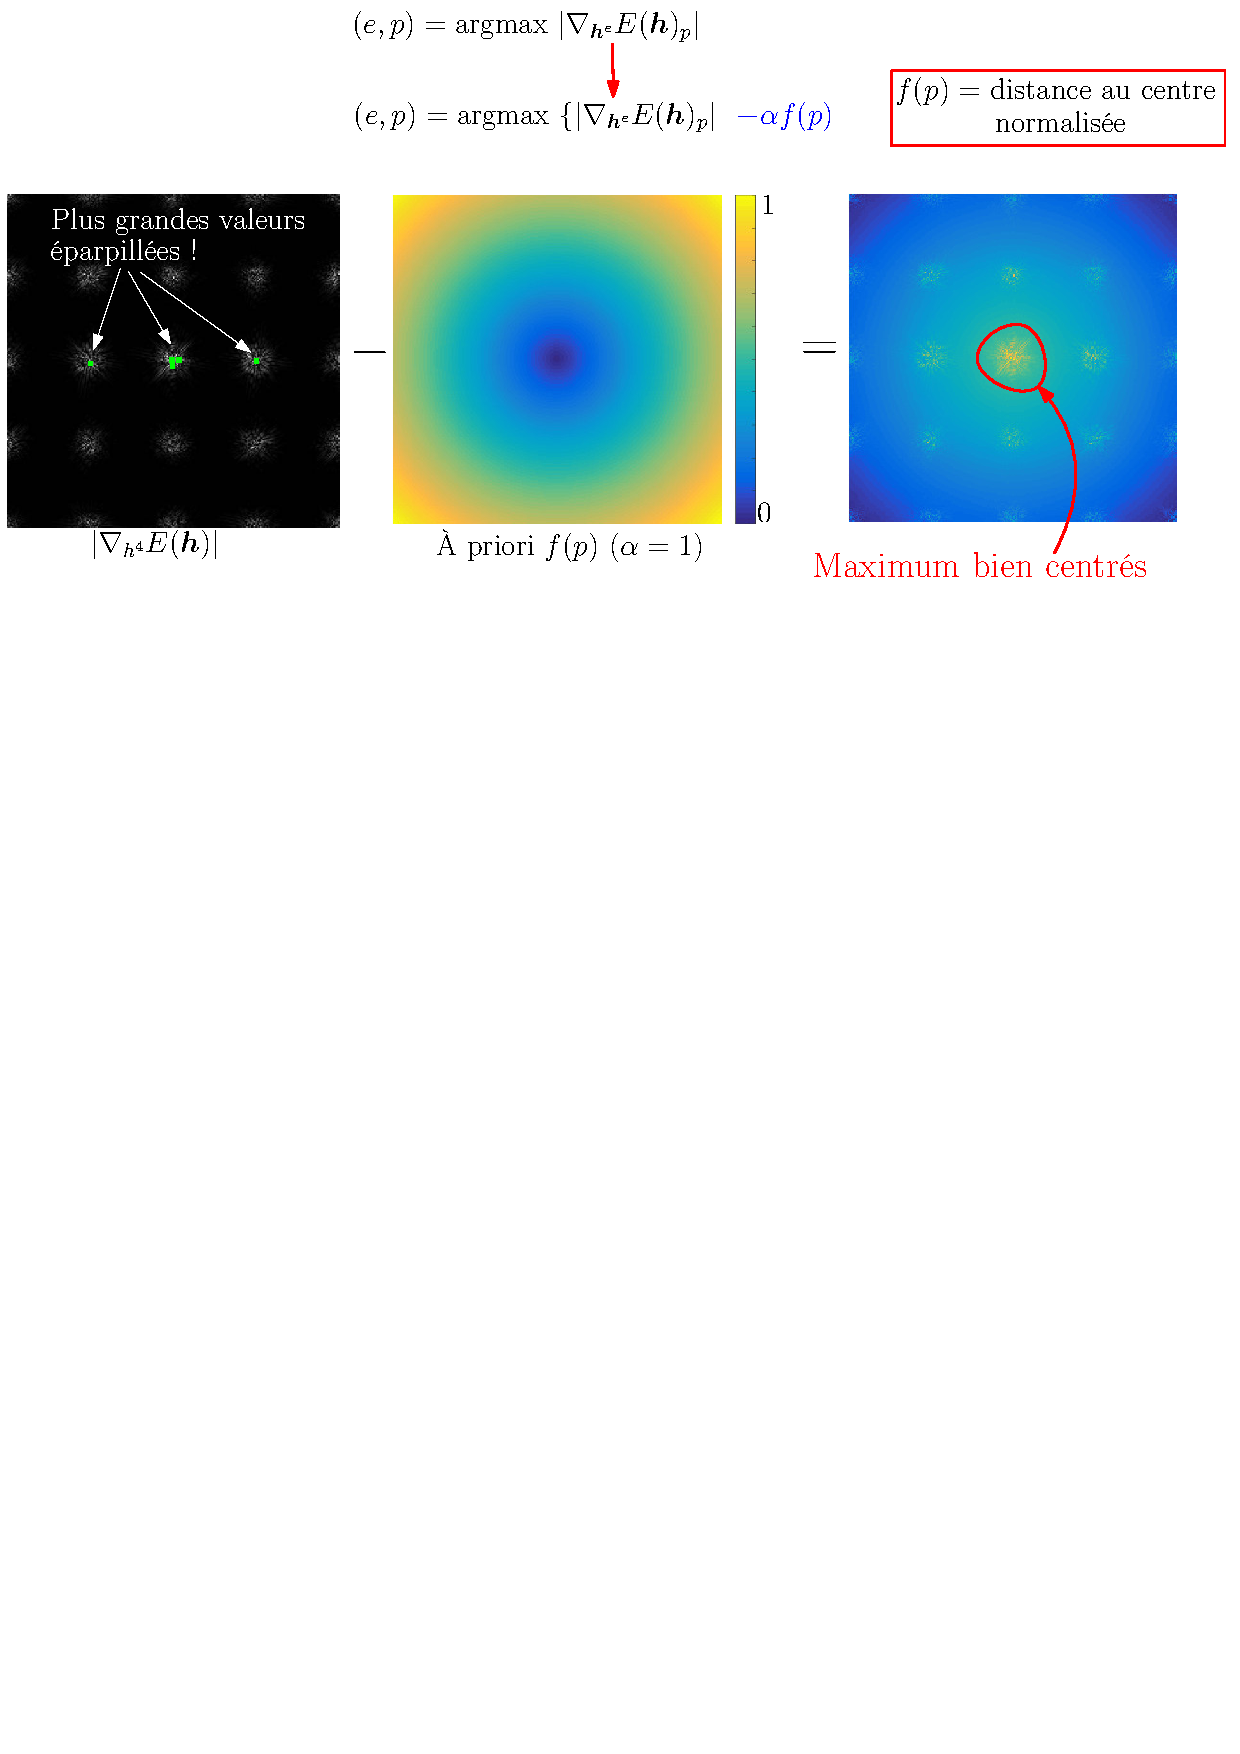
\includegraphics[width=1.1\linewidth]{figures/3-learn-tree-scattered/scattered-explication.pdf}}
\end{figure}
\begin{exampleblock}{} \centering 
Hyper-paramètre \alert{$\alpha$} à déterminer ?
\end{exampleblock}
\end{frame}


\begin{frame}{À priori $f$}
\begin{figure}\centering
    \makebox[\linewidth]{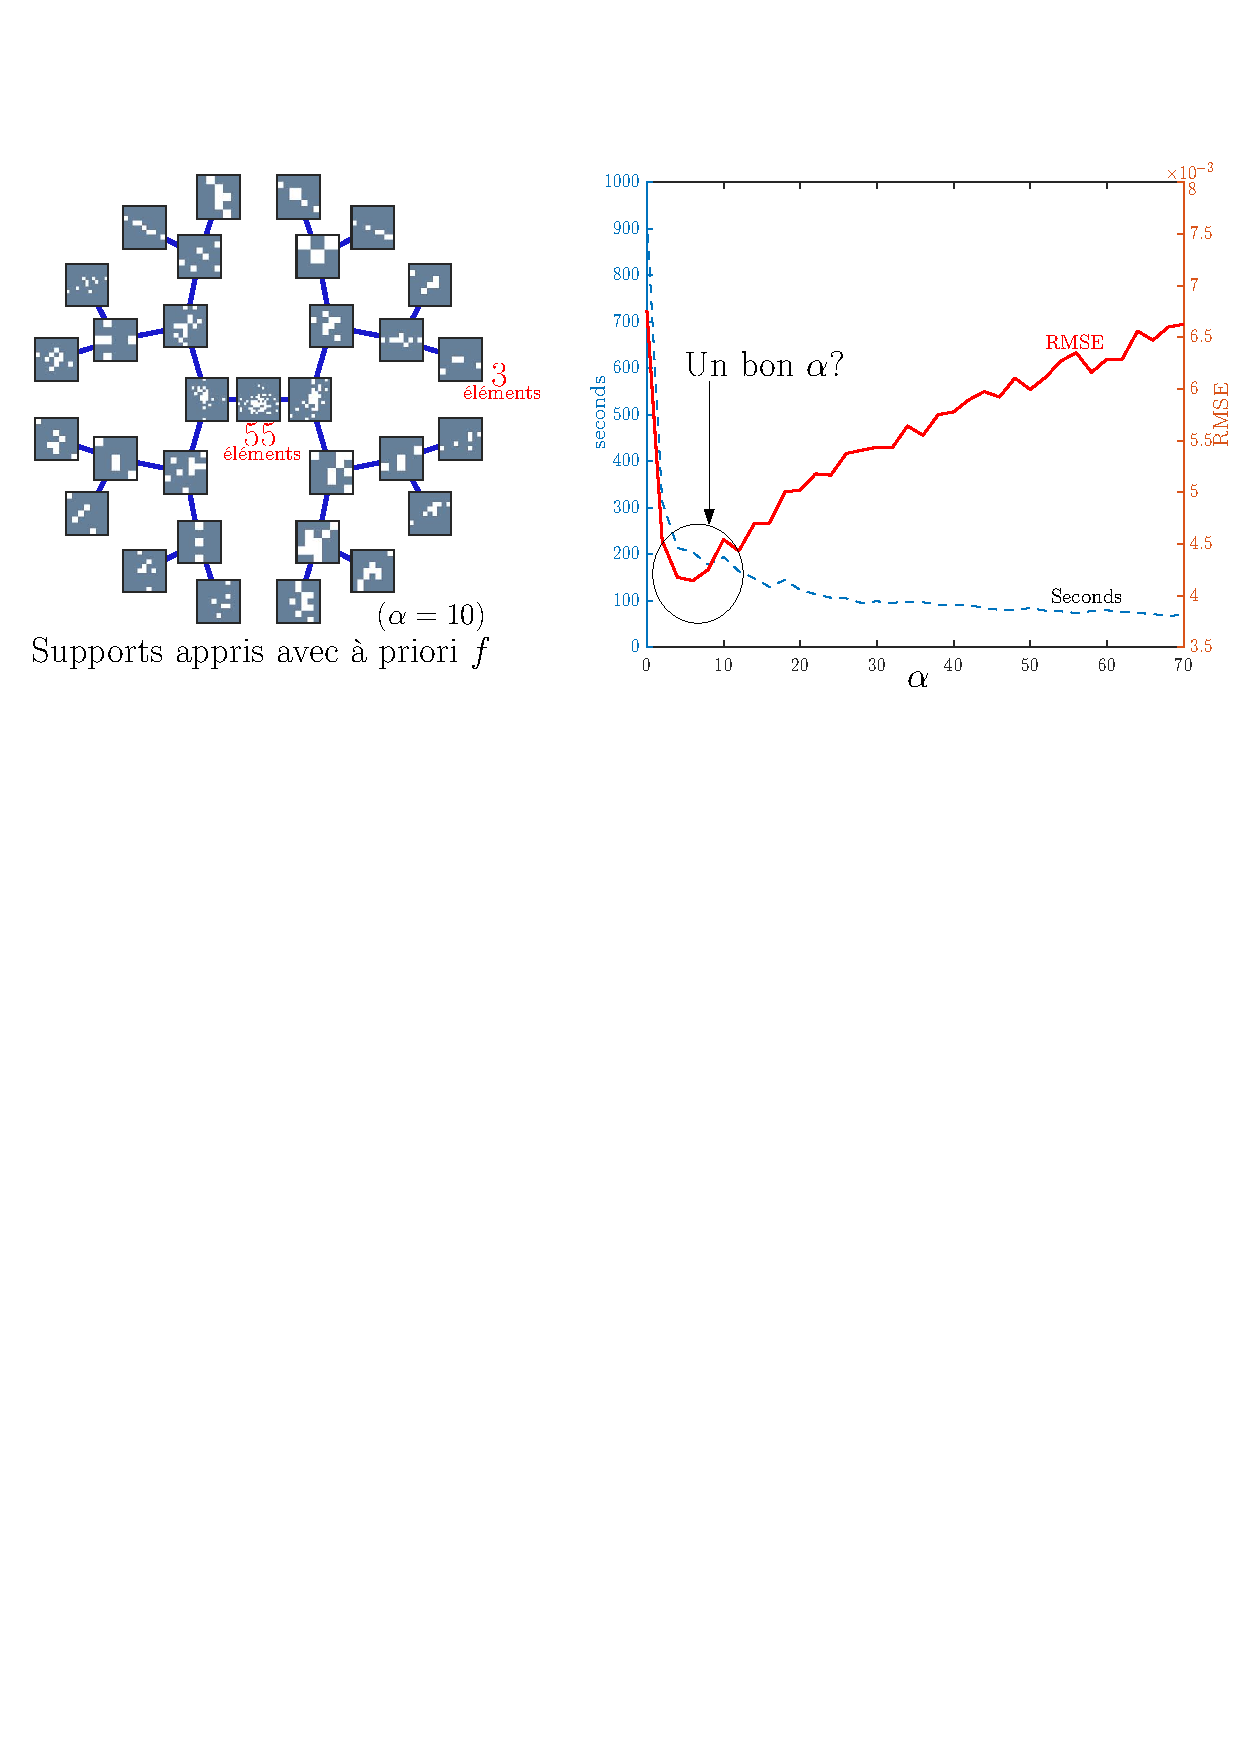
\includegraphics[width=1\linewidth]{figures/3-learn-tree-scattered/unscattered.pdf}}
\end{figure}
\end{frame}

\begin{frame}{Réglage de $\alpha$}
\begin{itemize}
\item Nous avons déterminé $\alpha$ au cas par cas
	\begin{figure}\centering
	    \makebox[\linewidth]{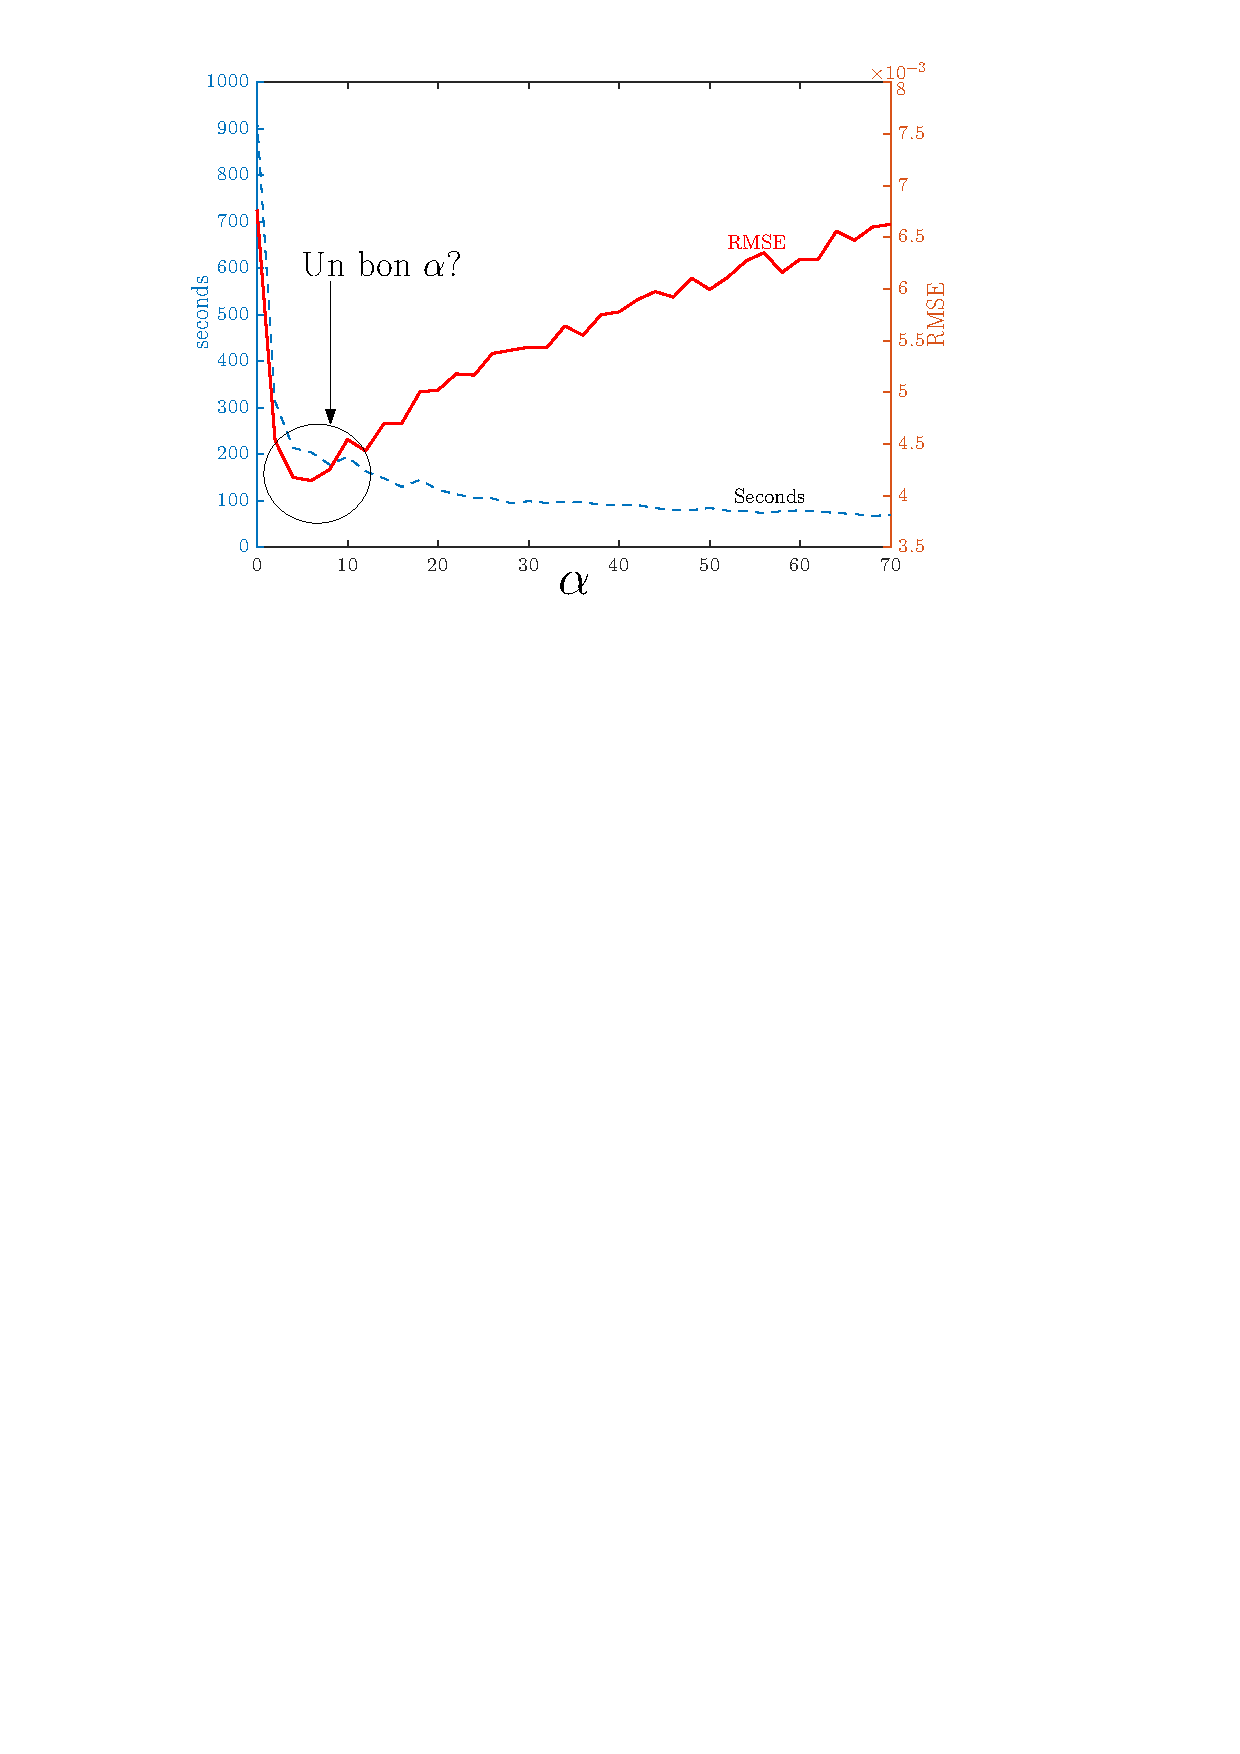
\includegraphics[width=0.8\linewidth]{figures/3-learn-tree-scattered/alpha.pdf}}
	\end{figure}
\item Déterminer $\alpha$ pendant OMP-PALMTREE : méthode SURE \cite{eldar_generalized_2009} ?
\end{itemize}
\end{frame}

\begin{frame}{Problème de déséquilibre avec à priori $f$}
\begin{itemize}
\item \alert{Déséquilibre :} 55 éléments au centre, 3 élément sur les feuilles
	\begin{figure}\centering
    \makebox[\linewidth]{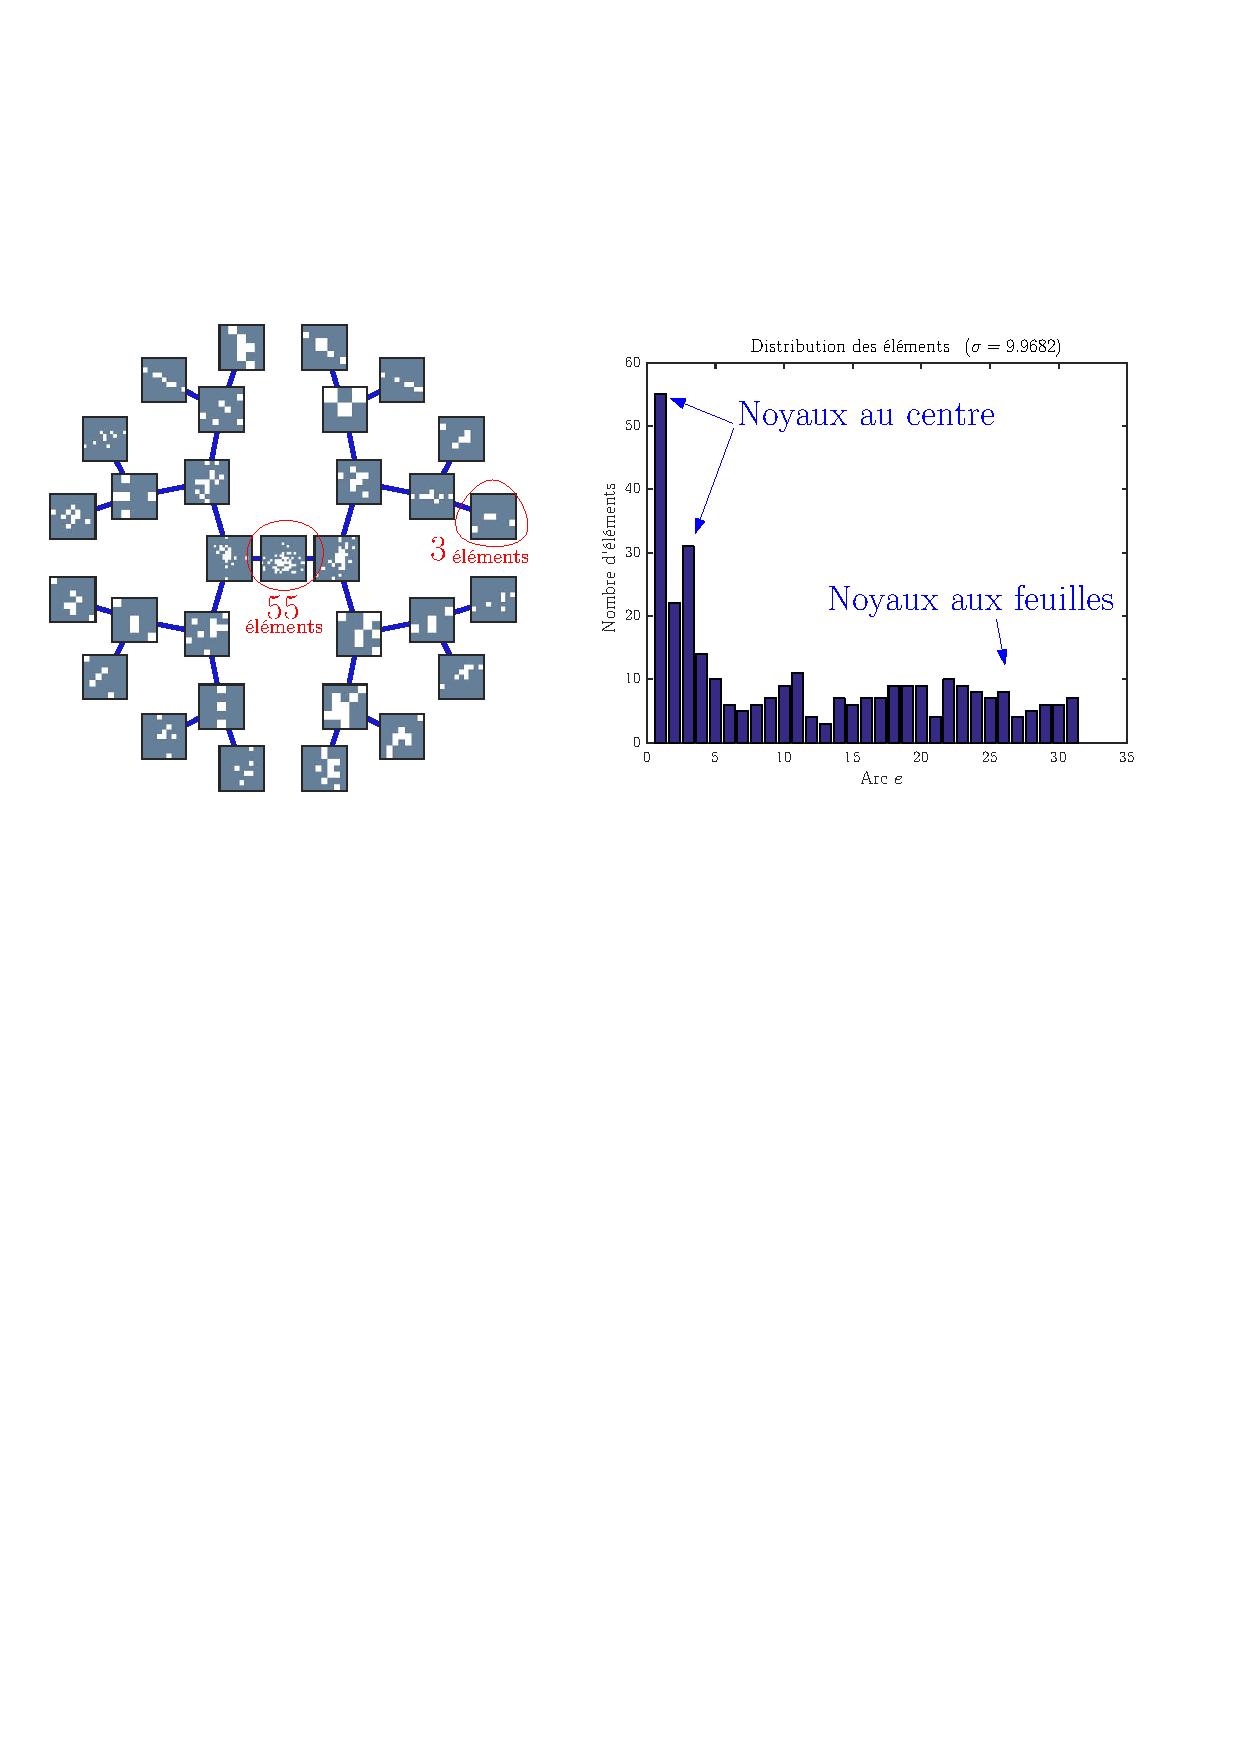
\includegraphics[width=1\linewidth]{figures/4-learn-tree-unbalanced/unbalanced.pdf}}
	\end{figure}
\item Trop d'éléments au centre $\rightarrow$ convolutions lentes (lié à l'implémentation)
\item Adapter $f(p)$ en fonction de l'arc $e$ ?

\end{itemize}
\end{frame}



\begin{frame}{Modification de la fonction d'à priori $f$ pour équilibrer}
\begin{figure}\centering
    \makebox[\linewidth]{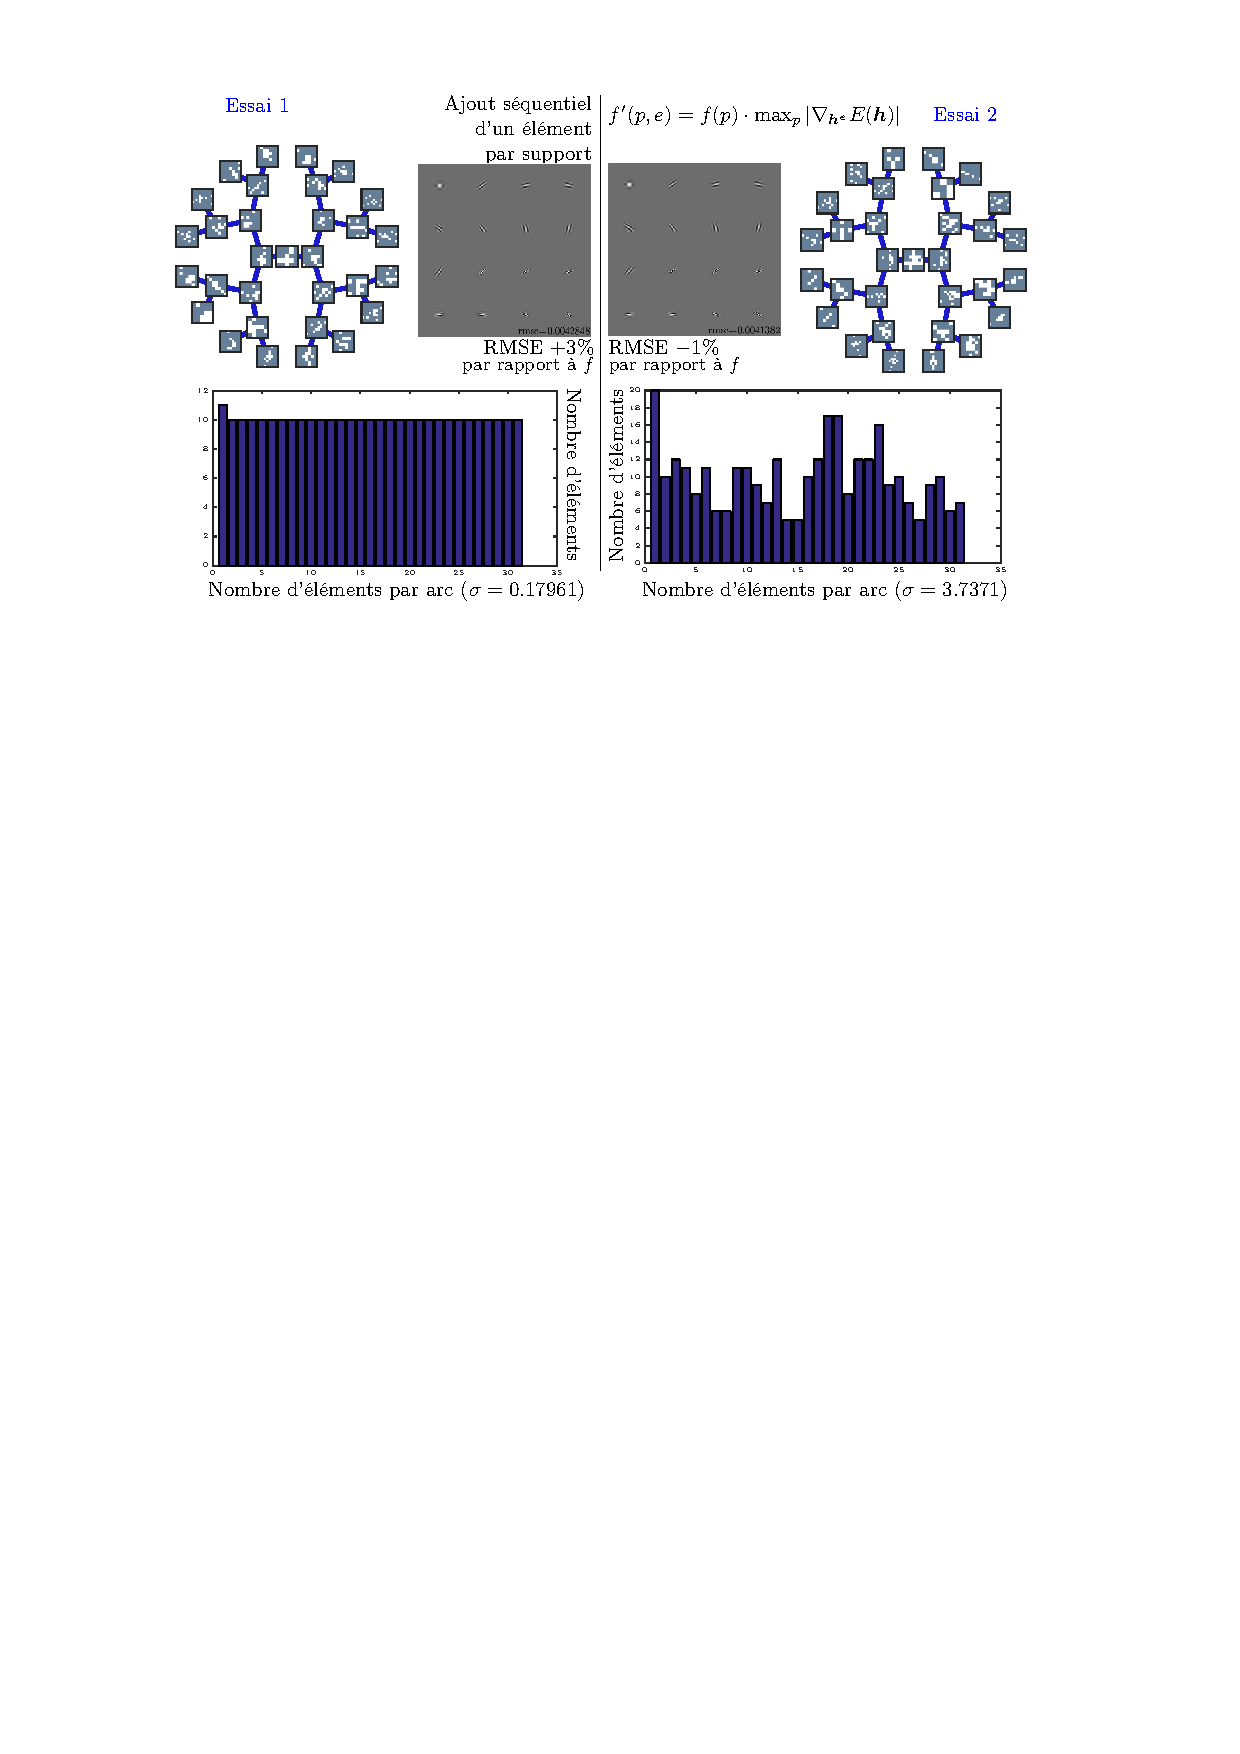
\includegraphics[width=1.1\linewidth]{figures/4-learn-tree-unbalanced/essai.pdf}}
\end{figure}
\end{frame}


\begin{frame}{Conclusions}

\begin{itemize}
\item[\cmark] \textbf{Verrou levé :} bon algorithme PALMTREE mais supports \alert{fixes} \\
	$\rightarrow$ \alert{estimation} des supports avec OMP-PALMTREE

\end{itemize}
Prochainement
\begin{itemize}
\item Estimer $\alpha$ à partir des données
\item Permettre la suppression d'éléments
\item Apprendre l'arbre

\end{itemize}
Pistes lointaines
\begin{itemize}
\item[\textcolor{purple}{\ding{43}}] Apprendre sur plusieurs images
\item[\textcolor{purple}{\ding{43}}] Passer à un algorithme minimisant à la fois $\D$ et $\x$
\end{itemize}
\vfill
\hfill Merci de votre attention
\end{frame}

\appendix

\backupbegin
\begin{frame}[allowframebreaks]
\frametitle{Bibliographie}
%\nocite{}
\printbibliography[heading=none]
\end{frame}
\backupend


\end{document}